 % -*- mode: LaTeX -*-
 % ... preamble ...
\documentclass[times,12pt,titlepage]{mstthesis}
\doublespacing
\usepackage{threeparttable}
\usepackage[final]{graphicx}
\usepackage{psfrag}
\usepackage{listings}
\usepackage{minted}
\usepackage[noprefix]{nomencl}
\usepackage{subcaption}
\usepackage{xr}
\usepackage{rotating}
\makenomenclature
\renewcommand{\nomgroup}[1]{
   \ifthenelse{\equal{#1}{A}}{\medskip \item \textbf{Roman}}{}%
   \ifthenelse{\equal{#1}{G}}{\medskip \item \textbf{Greek}}{}%
   \ifthenelse{\equal{#1}{S}}{\medskip \item \textbf{Subscripts}}{}%
}
\usepackage[nopar]{lipsum} % ... provides dummy text ...

 % ... end preamble ...

\begin{document}

 % ... specify: ms or phd ...

\begin{ThesisTitlePage}{phd}

 % ... title page info ...

\author{\MakeUppercase{Edward T. Norris}}

\thesistitle{\MakeUppercase{Discrete Ordinates CT Organ Dose Simulator (DOCTORS)}}

\department{Nuclear Engineering}

 % ... thesis committee ...

\ThesisAdviser{Xin Liu}

 % If you have a co-advisor, enter the name in the
 % curly braces below and uncomment.
 % Otherwise, leave commented out.
 %\cothadviser{} % If you have 2 thesis advisers

\memberone{Ayodeji Alajo}
\membertwo{Hyoung Koo Lee}
\memberthree{Gary Mueller}
\memberfour{Fikret Ercal}
%\memberfive{Prandtl}

 % ... Graduation date - NOT your submission date ...
\graddate{2017}

\end{ThesisTitlePage}
 % ... copyright page - true|false ...

\copyrightyear{2017}
\ThesisCopyrightPage{true}

 % ... front matter - thesis abstract ...

\begin{ThesisAbstract}
This is the text for the abstract. Here, I explain what I did and how cool I am for doing it. Because I am awesome.

Computed tomography (CT) has become pervasive in medical diagnostics as improved imaging techniques and processing algorithms provide higher quality information to doctors. However, the exponentially increasing usage of CT has raised concerns regarding long term low-dose radiological risks. Currently, the dose to patients is computed using Monte Carlo methods and experimental tests. In other areas of radiation transport, deterministic codes have been shown to be much faster than Monte Carlo codes.

Currently, no deterministic methodology exists to automatically generate a spatially distributed dose profile from a CT voxel phantom. This work proposes a new code, Discrete Ordinate CT Organ Dose Simulator (DOCTORS) which utilizes a GPU accelerated raytracer and discrete ordinate solver to compute photon flux in the patient. The flux is then converted to dose.

The DOCTORS code was benchmarked against MCNP6 and found to have very good agreement using both a water phantom and a realistic patient phantom. DOCTORS was also found to be much faster than MCNP6, even more so with GPU acceleration.

GPU

\end{ThesisAbstract}

 % ... front matter - thesis acknowledgements ...

\begin{ThesisAcknowledgment}
I would like to thank my adviser, Dr. Liu and all of the other graduate students for their continued support through my graduate career. I also appreciate the time spent by my committee members helping me identify problems and provide insight to solutions. 

I would also like to acknowledge the NRC for providing funding for my work. My work is supported by NRC grant NRC-HQ-13-G-38-0026.
\end{ThesisAcknowledgment}

\begin{ThesisFrontMatter}
\tableofcontents
\listoffigures
\listoftables
\listofsymbols
\end{ThesisFrontMatter}

\begin{ThesisBody}

 % ... introduction chapter ...
\ThesisBodyChapter{Introduction}%%
%% This is file `chapmin.tex',
%% generated with the docstrip utility.
%%
%% The original source files were:
%%
%% ths.dtx  (with options: `chapmin')
%% 
%% IMPORTANT NOTICE:
%% 
%% For the copyright see the source file.
%% 
%% Any modified versions of this file must be renamed
%% with new filenames distinct from chapmin.tex.
%% 
%% For distribution of the original source see the terms
%% for copying and modification in the file ths.dtx.
%% 
%% This generated file may be distributed as long as the
%% original source files, as listed above, are part of the
%% same distribution. (The sources need not necessarily be
%% in the same archive or directory.)


Computed tomography (CT) is becoming increasingly pervasive in medical diagnostics because improved algorithms are giving doctors more access to patient information. Increased information results in faster and more accurate diagnosis. However, the CT operation itself gives a radiation dose to the patient which carries some associated risk. A more detailed measure of that risk would help doctors make informed decisions regarding whether a CT scan is warannted, and if so, which type. This can also help doctors estimate spatial dose distribution to the patient to ensure no specific organ received more dose than permissible.

Another application is in treatment.

Currently, no algorithm exists to provide this information.

The goal of this work is to provide such an algorithm.

There are two primary avaialble for the methodologies: Monte Carlo and deterministic methods. Monte Carlo has proven to be very slow in these areas. Furhter, the 3D Cartesian mesh generated from CT reconstruction is well suited to deterministic computation. 

This work forcuses on the discrete ordinates method and presents an implementation specially developed for dose estimation from a medical CT scan. 

Computational mesh from a sinogram. Reconstruction.

\endinput
%%
%% End of file `chapmin.tex'.

 % ... chapter ...
\ThesisBodyChapter{Literature Review}%%
%% This is file `chapbib.tex',
%% generated with the docstrip utility.
%%
%% The original source files were:
%%
%% ths.dtx  (with options: `chapmin,addbib')
%% 
%% IMPORTANT NOTICE:
%% 
%% For the copyright see the source file.
%% 
%% Any modified versions of this file must be renamed
%% with new filenames distinct from chapbib.tex.
%% 
%% For distribution of the original source see the terms
%% for copying and modification in the file ths.dtx.
%% 
%% This generated file may be distributed as long as the
%% original source files, as listed above, are part of the
%% same distribution. (The sources need not necessarily be
%% in the same archive or directory.)

This chapter summarizes the literature reviewed in preparation of this work. The literature review is split into multiple sections, each highlighting relevant works pertaining to a particular component or section of this work. The first two sections cover introductory work and steps necessary for preprocessing data. Section~\ref{sec:discordlit} covers historical and recent work in discrete ordinate solution methodology, the methodology used by DOCTORS. The remaining sections cover GPU hardware and other implementation facets.

\section{CT Dose Estimation}
The dose a patient receives form both diagnostic CT procedures and radiation therapy is of great concern to the medical community [CITE]. 

MOTIVATION

Monte Carlo codes have been used in the past to compute flux-to-dose conversion factors for a reference person [CITE ICRP].

Dose estimations have been made using many methodologies including 

COMPUTATION

\section{CT Phantom Generation}
The CT phantom is populated with CT numbers, also known as Hounsfield numbers. These values are related to the attenuation coefficient of the material represented by the voxel. Traditionally, a CT number of zero corresponds to the attenuation of water while -1000 corresponds to dry air CITE though some variations do exist CITE.

Many authors have provided correlations that map the CT number to both a material and a density.

First ones.
Saw \citep{ref:sawc} did stuff. And \citep{ref:plessisf}. Then \citet{ref:schneideru} said stuff. And \citet{ref:kimh} did stuff with GEANT4.

Another Schneider did some stuff too \citep{ref:schneiderw}. And Vanderstraeten has a long name \citep{ref:vanderstraetenb}.

The new guy provides 19 materials. The density is measured.
The DOCTORS code relies on the CT nuber to material mapping of \citet{ref:ottossonr} who developed a 19-group BLAH. Table~\ref{table:ctmap} shows the mapping of CT number to material composition (reproduced from \citep{ref:ottossonr}).

\begin{sidewaystable}[ht]
\caption{Water Regions}
\centering 
\begin{tabular}{l c r r r r r r r r r r r r}
\hline \hline   
Media       & CT Range      & H    & C    & N    & O    & Na  & Mg  & P    & S   & Cl  & Ar  & K   & Ca \\ [0.5ex] 
\hline
Air         & -950 to -100  &      &      & 75.7 & 23.3 &     &     &      &     &     & 1.3 &     &      \\
Lung        & -1000 to -950 & 10.3 & 10.5 &  3.1 & 74.9 & 0.2 &     &  0.2 & 0.3 & 0.3 &     & 0.2 &      \\
Adipose     & -100 to 15    & 11.2 & 50.8 &  1.2 & 36.4 & 0.1 &     &      & 0.1 & 0.1 &     &     &      \\
Connective  & 15 to 129     & 10.0 & 16.3 &  4.3 & 68.4 & 0.4 &     &      & 0.4 & 0.3 &     &     &      \\
Bone 1      & 129 to 200    &  9.7 & 44.7 &  2.5 & 35.9 &     &     &  2.3 & 0.2 & 0.1 &     & 1.0 &  4.5 \\ 
Bone 2      & 200 to 300    &  9.1 & 41.4 &  2.7 & 36.8 &     & 0.1 &  3.2 & 0.2 & 0.1 &     & 1.0 &  6.3 \\ 
Bone 3      & 300 to 400    &  8.5 & 37.8 &  2.9 & 37.9 &     & 0.1 &  4.1 & 0.2 & 0.1 &     & 1.0 &  8.2 \\ 
Bone 4      & 400 to 500    &  8.0 & 34.5 &  3.1 & 38.8 &     & 0.1 &  5.0 & 0.2 & 0.1 &     & 1.0 & 10.0 \\ 
Bone 5      & 500 to 600    &  7.5 & 31.6 &  3.2 & 39.7 &     & 0.1 &  5.8 & 0.2 & 0.1 &     &     & 11.6 \\ 
Bone 6      & 600 to 700    &  7.1 & 28.7 &  3.4 & 40.4 &     & 0.1 &  6.6 & 0.2 & 0.1 &     &     & 13.1 \\ 
Bone 7      & 700 to 800    &  6.7 & 26.7 &  3.5 & 41.2 &     & 0.2 &  7.2 & 0.3 &     &     &     & 14.4 \\ 
Bone 8      & 800 to 900    &  6.3 & 24.7 &  3.7 & 41.8 &     & 0.2 &  7.8 & 0.3 &     &     &     & 15.7 \\ 
Bone 9      & 900 to 1000   &  6.0 & 22.7 &  3.8 & 42.4 &     & 0.2 &  8.4 & 0.3 &     &     &     & 16.8 \\ 
Bone 10     & 1000 to 1100  &  5.6 & 20.7 &  3.9 & 43.0 &     & 0.2 &  8.9 & 0.3 &     &     &     & 17.9 \\ 
Bone 11     & 1100 to 1200  &  5.3 & 18.7 &  4.0 & 43.5 &     & 0.2 &  9.4 & 0.3 &     &     &     & 18.9 \\ 
Bone 12     & 1200 to 1300  &  5.1 & 16.7 &  4.1 & 44.0 &     & 0.2 &  9.9 & 0.3 &     &     &     & 19.8 \\
Bone 13     & 1300 to 1400  &  4.8 & 15.7 &  4.2 & 44.4 &     & 0.2 & 10.3 & 0.3 &     &     &     & 20.7 \\
Bone 14     & 1400 to 1500  &  4.6 & 13.7 &  4.2 & 44.9 &     & 0.2 & 10.7 & 0.3 &     &     &     & 21.5 \\  
Bone 15     & > 1500        &  4.3 & 12.7 &  4.3 & 45.3 &     & 0.2 & 11.1 & 0.3 &     &     &     & 22.2 \\[1ex]
\hline
\end{tabular}
\label{table:ctmap}
\end{sidewaystable}

Two phantom datasets are used in this work [CITE].

\section{Discrete Ordinates}\label{sec:discordlit}
The dsicrete ordinates method dates back to CITE but remains one of the most prominent solution modalities for ration transport in use today.

A comprehensive review of discrete ordinate methods is given by \citet{ref:lewise}. Additional references include 

Monte Carlo codes such as TOPAS and Geant4 \citep{ref:agostinellis} are the gold standard \citep{ref:jiax}

Codes such as EGS4, its improved versions EGSnrc, and EGS5 \citep{ref:nelsonw}, and PENELOPE \citep{ref:salvatf} are all Monte Carlo and have shown very good results to experimental. But they are developed for high energy physics.


The Exnihilo thing by \citet{ref:evanst}. And DeHart wrote in \citep{ref:dehartm}

The Ibrahim did stuff \citep{ref:ibrahima} and Lee did stuff too \citep{ref:leeb}.

With regards to angles, stuff has been done \citep{ref:ahrensc}

There are many acceleration techniques available for discrete ordinates \citep{ref:efremenkod} that can increase speed by 15-30\%.

GPU methods exist for solar stuff at satellites.

The geometry has been extended to Non-Uniform Rational B-Splins (NURBS) for reactor eigenvalue problems.

Attila had a 1st col src added by \citep{ref:wareingt}. Some rays are better than others \citep{ref:mathewsk}.

Dort and Tort \citep{ref:rhoadesw}.

Denovo.

\section{Raytracing}

Raytracing is important too. Woo came up with on \citep{ref:wooa} which was improved by \citet{ref:liuy} and \citet{ref:hel}.

\section{GPU Acceleration}

Monte Carlo dose computation for protons has been accelerated by GPU technology \citep{ref:jiax} and 

Monte Carlo in voxelized geometries has been done by \citep{ref:hissoinys} for monoenergetic beams.
GPUs are cool.

CUDA is cool.


\endinput
%%
%% End of file `chapbib.tex'.

 % ... chapter ...
\ThesisBodyChapter{Methods}%%
%% This is file `chapmin.tex',
%% generated with the docstrip utility.
%%
%% The original source files were:
%%
%% ths.dtx  (with options: `chapmin')
%% 
%% IMPORTANT NOTICE:
%% 
%% For the copyright see the source file.
%% 
%% Any modified versions of this file must be renamed
%% with new filenames distinct from chapmin.tex.
%% 
%% For distribution of the original source see the terms
%% for copying and modification in the file ths.dtx.
%% 
%% This generated file may be distributed as long as the
%% original source files, as listed above, are part of the
%% same distribution. (The sources need not necessarily be
%% in the same archive or directory.)


\section{Mathmatic Development}

Where does this text go?

\subsection{The Boltzmann Equation}

The time dependent gamma transport equation can be written as

\begin{equation} \label{eq:boltz_t_dep}
\begin{split}
	&\left[ \frac{1}{v(E)} \frac{\partial}{\partial t} + \hat{\Omega} \cdot \nabla + \Sigma_t(\boldsymbol{r}, E, t) \right]
	\psi(\boldsymbol{r}, E, \hat{\Omega}, t) = \\
	&\int_{4 \pi} \int_0^\infty \Sigma_s(\boldsymbol{r}, E' \rightarrow E, \hat{\Omega}' \rightarrow \hat{\Omega}, t) \psi(\boldsymbol{r}, E', \hat{\Omega}', t) dE' d\hat{\Omega}' + S(\boldsymbol{r}, E, \hat{\Omega}, t)
\end{split}
\end{equation}

However, we are typically not concerned with the transient case in medical diagnostic imaging. We are more interested in the steady state case. The time independent form of Eq. \ref{eq:boltz_t_dep} is written as

\begin{equation} \label{eq:boltz}
\begin{split}
	&\left[ \hat{\Omega} \cdot \nabla + \Sigma_t(\boldsymbol{r}, E) \right]
	\psi(\boldsymbol{r}, E, \hat{\Omega}) = \\
	&\int_{4 \pi} \int_0^\infty \Sigma_s(\boldsymbol{r}, E' \rightarrow E, \hat{\Omega}' \rightarrow \hat{\Omega}) \psi(\boldsymbol{r}, E', \hat{\Omega}') dE' d\hat{\Omega}' + S(\boldsymbol{r}, E, \hat{\Omega})
\end{split}
\end{equation}

The following sections show how Eq.~\ref{eq:boltz} is discretized.

\subsection{Angular Discretization}
The coordinate system used in DOCTORS is shown in Fig.~\ref{fig:coord_sys}. A discrete set of $N_a$ angles ($\Omega_{a} \quad a = 0 \ldots N_a-1$) is selected to represent continuous directional space. Particles are transported only along these discrete directions form one voxel to adjacent voxels.

The rotation symmetrical quadrature is implemented in DOCTORS. There are many different quadrature sets, the rotation symmetrical quadratures were selected because they are easy to implement, rotationally symmetric, and the most commonly used in production discrete ordinate solvers. This enables simple, direct comparison to other solvers. Arbitrary quadratures are permissible in a plain text file supplied by the user enabling other quadratures.

\begin{figure}[tb]
  \begin{center}
   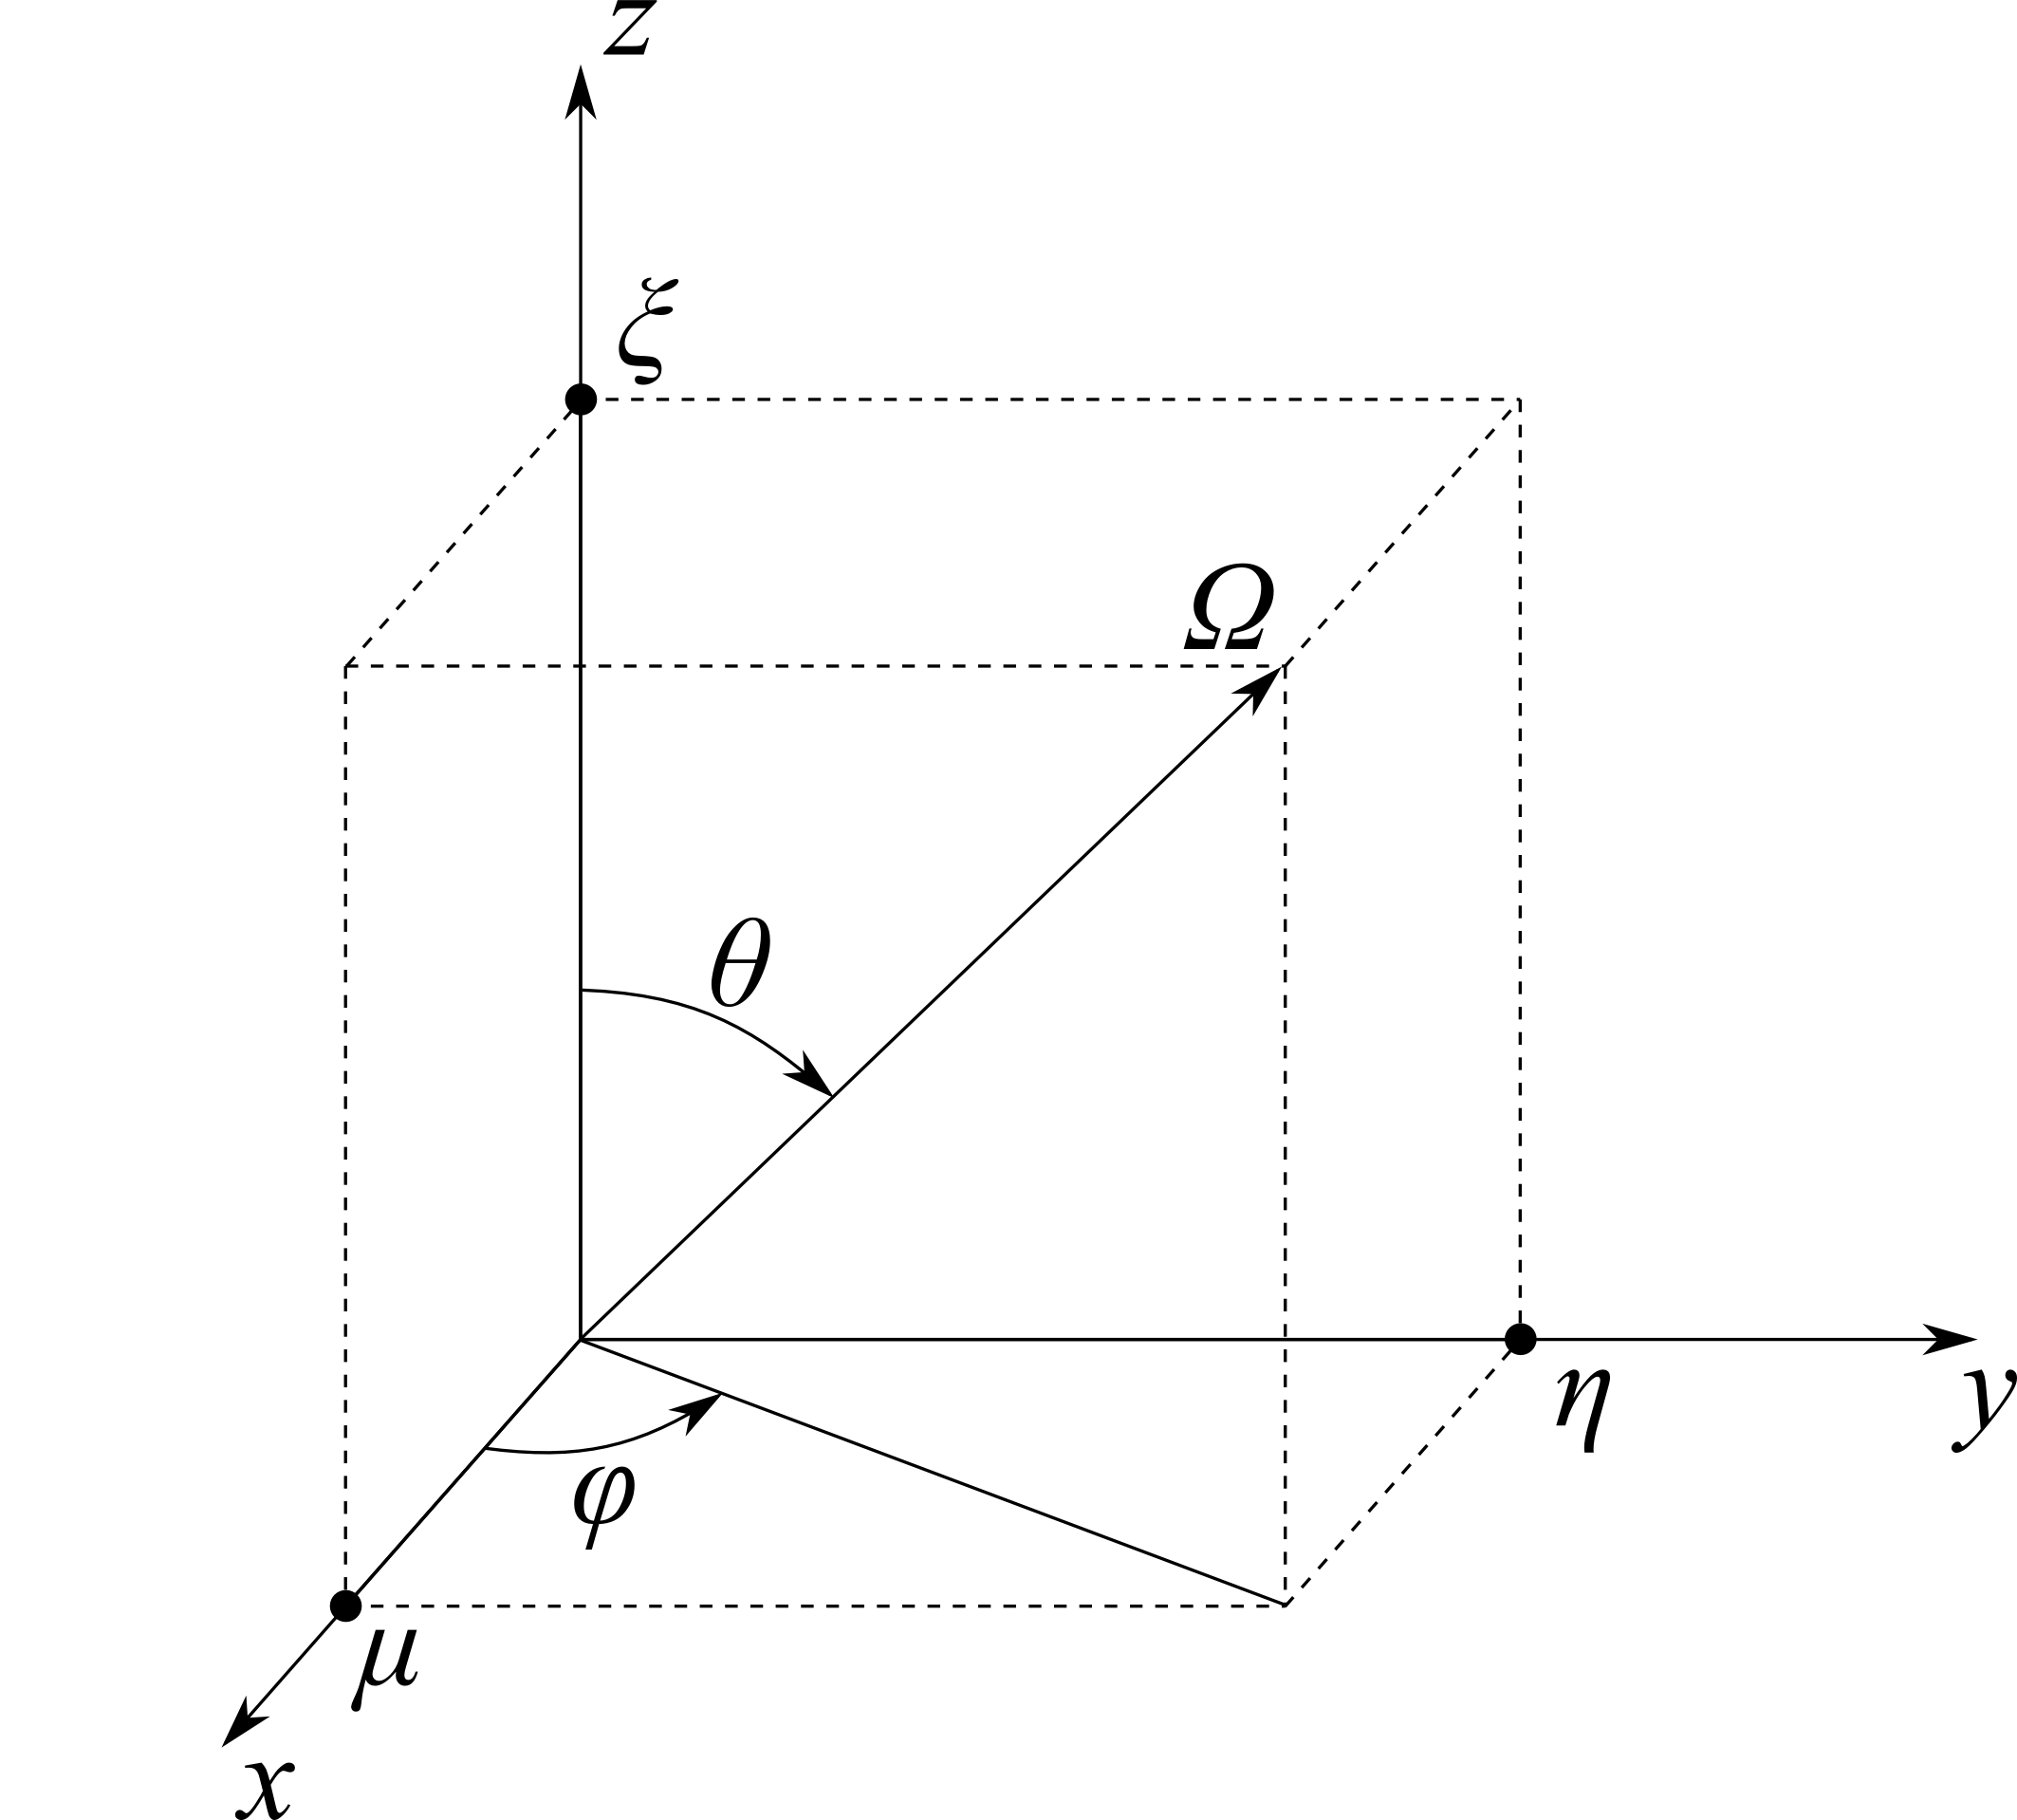
\includegraphics[width=3.75in]{figs/coord_sys}
  \end{center}
  \caption{The coordinate system used in DOCTORS. Given an arbitrary direction, $\Omega$, $\mu$, $\eta$, and $\xi$ are its direction cosines with respect to the $x$, $y$, and $z$ axes respectively. $\varphi$ is the azimuthal angle (with respect to $x$ and the d $\theta$ is the polar angle (with respect to $z$).}
\label{fig:coord_sys}
\end{figure}%

A given direction, $\hat{\Omega}$ is determined by its three cosine components. This relation is given in Eq.~\ref{eq:omega_cos} where $\hat{i}$, $\hat{j}$, and $\hat{k}$ are the unit directions in the $x$, $y$, and $z$ directions respectively.

\begin{equation} \label{eq:omega_cos}
	\hat{\Omega} = \mu \hat{i} + \eta \hat{j} + \xi \hat{k}
\end{equation}

Each discrete angle is associated a weight. The weights are designed with the angles such that once a discrete quadrature is selected, integration over continuous space becomes integration in discrete space approximated by Eq.~\ref{eq:disc_int}.

\begin{equation} \label{eq:disc_int}
\int_{4 \pi} f(\hat{\Omega}) d\Omega \approx \sum_{a=0}^{N_a-1} f(\hat{\Omega}_a) \omega_a
\end{equation}

Discretizing Eq.~\ref{eq:boltz} in angular space gives Eq.~\ref{eq:boltz_a} where the angle is denoted by subscript $a$.

\begin{equation} \label{eq:boltz_a}
\begin{split}
&\left[ \hat{\Omega}_a \cdot \nabla + \Sigma_t(\boldsymbol{r}, E) \right]
\psi_{a}(\boldsymbol{r}, E) = \\
&\sum_{a=0}^{N_a-1} \int_0^\infty \Sigma_{s, a, a'}(\boldsymbol{r}, E' \rightarrow E) \psi_{a'}(\boldsymbol{r}, E') dE' \omega_a + S_a(\boldsymbol{r}, E)
\end{split}
\end{equation}

\subsection{Energy Discretization}

Continuous energy is discretized into $G$ groups indexed from 0 to $G-1$. Upscatter is assumed to be negligible. Therefore, Eq.~\ref{eq:boltz_a} becomes the energy discretized Eq.~\ref{eq:boltz_e} where the group number is indexed by superscript $g$. The group structure is shown in Fig.~\ref{fig:energy_groups}.

\begin{equation} \label{eq:boltz_e}
\left[ \hat{\Omega}_a \cdot \nabla + \Sigma_t^g(\boldsymbol{r}) \right]
\psi_{a}^{g}(\boldsymbol{r}) = 
\sum_{a=0}^{N_a-1} \sum_{g'=g}^{G-1} \Sigma_{s, a, a'}^{g, g'}(\boldsymbol{r}) \psi_{a'}^{g'}(\boldsymbol{r}) \omega_a + S_a^g(\boldsymbol{r})
\end{equation}

\begin{figure}[tb]
  \begin{center}
   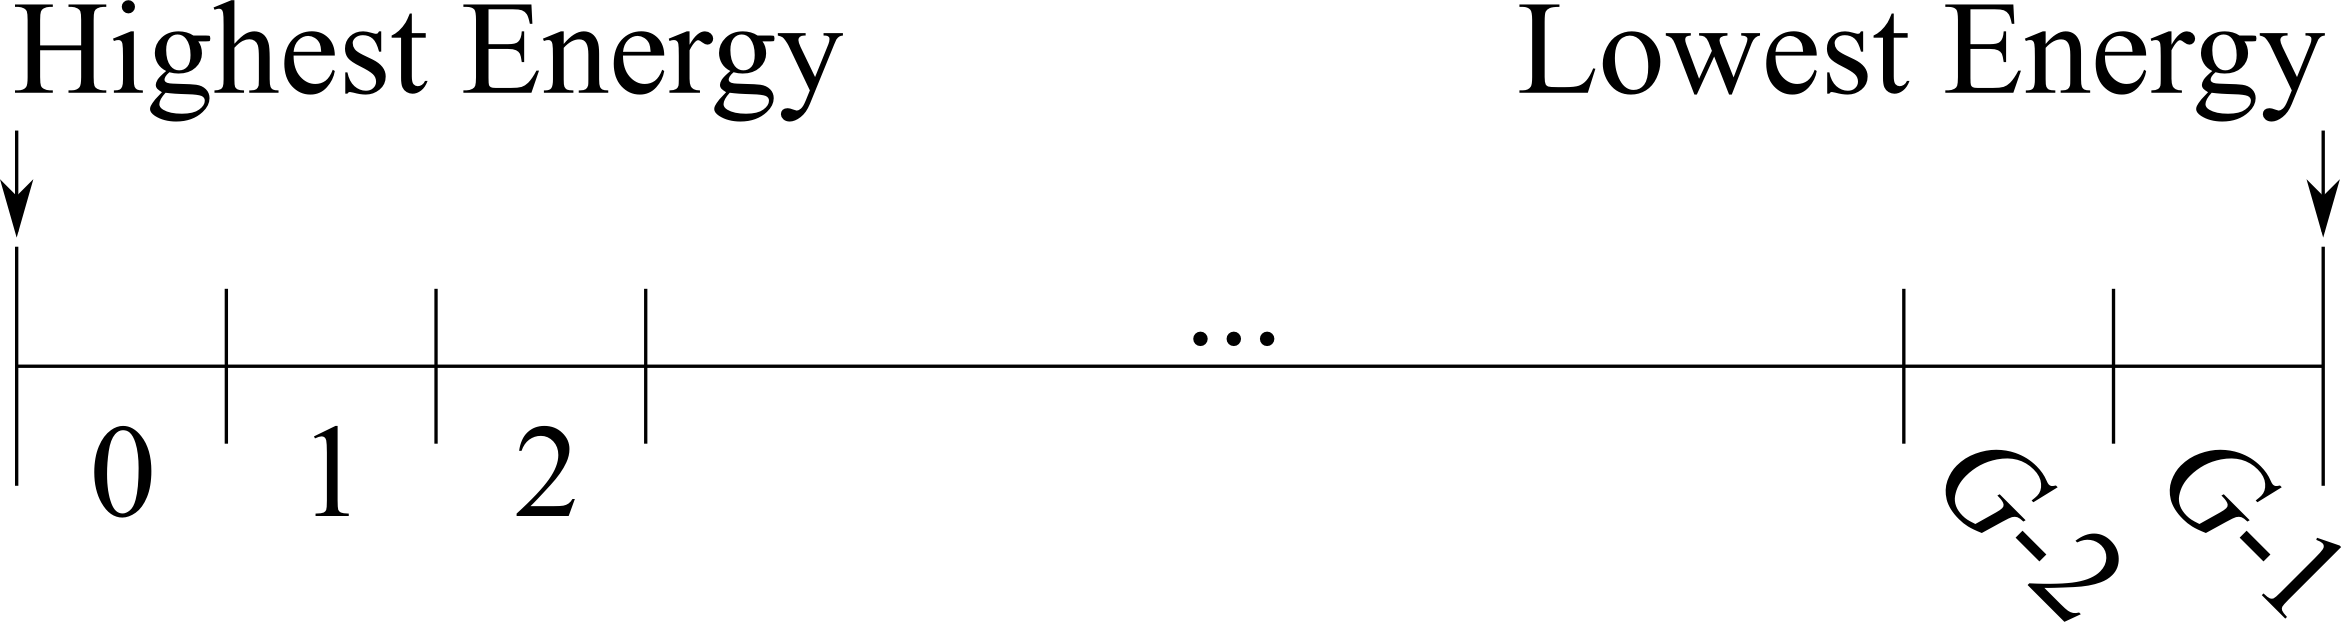
\includegraphics[width=3.75in]{figs/energy_groups}
  \end{center}
  \caption{The energy grid structure used in DOCTORS. The highest energy group is group 0 and the lowest energy is group $G-1$.}
\label{fig:energy_groups}
\end{figure}%

\subsection{Cross Section Parsing}
AMPX cross sections are read in binary. They are formatted like so. They are read like so. They were obtained from SCALE6.2. These files can be generated by other codes.

\subsection{Spatial Discretization}

Finally, Eq.~\ref{eq:boltz_e} is discretized in space to give Eq.~\ref{eq:boltz_i} which is fully discretized. The problem domain is split into an evenly spaced Cartesian grid. The grid spacing between each of the spatial dimensions does not necessarily need to be uniform, but it often is in the case of CT voxel phantoms.

The problem domain must be a regular rectangular parallelpiped of size $D_x$, $D_y$, and $D_z$ in the $x$, $y$, and $z$ directions respectively. The mesh is partitioned into $N_x$, $N_y$, and $N_z$ evenly spaced bins along each direction. The total number of voxels, $N_V$ is easily computed as the multiple of each of the component directions given in Eq.~\ref{eq:n_v}.

\begin{equation} \label{eq:n_v}
	N_V = N_x N_y N_z
\end{equation}

Voxel indices are reordered into a one dimensional vector (flattened) according to the rule given in Eq.~\ref{eq:indx_flat}. Note that indices start at zero.

\begin{equation} \label{eq:indx_flat}
	i = i_x (N_z + N_y) + i_y N_z + i_z
\end{equation}

The spatial mesh is shown in Fig.~\ref{fig:spatial_disc}. The size of each voxel in each dimension is computed by dividing the size of the problem domain along in that dimension by the number of mesh elements along the same direction. Eq.~\ref{eq:mesh_x} shows this computation for the $x$ direction. Analagous equations apply in the $y$ and $z$ directions as well.

\begin{equation} \label{eq:mesh_x}
\Delta x = \frac{D_x}{N_x}
\end{equation}

\begin{figure}[tb]
  \begin{center}
   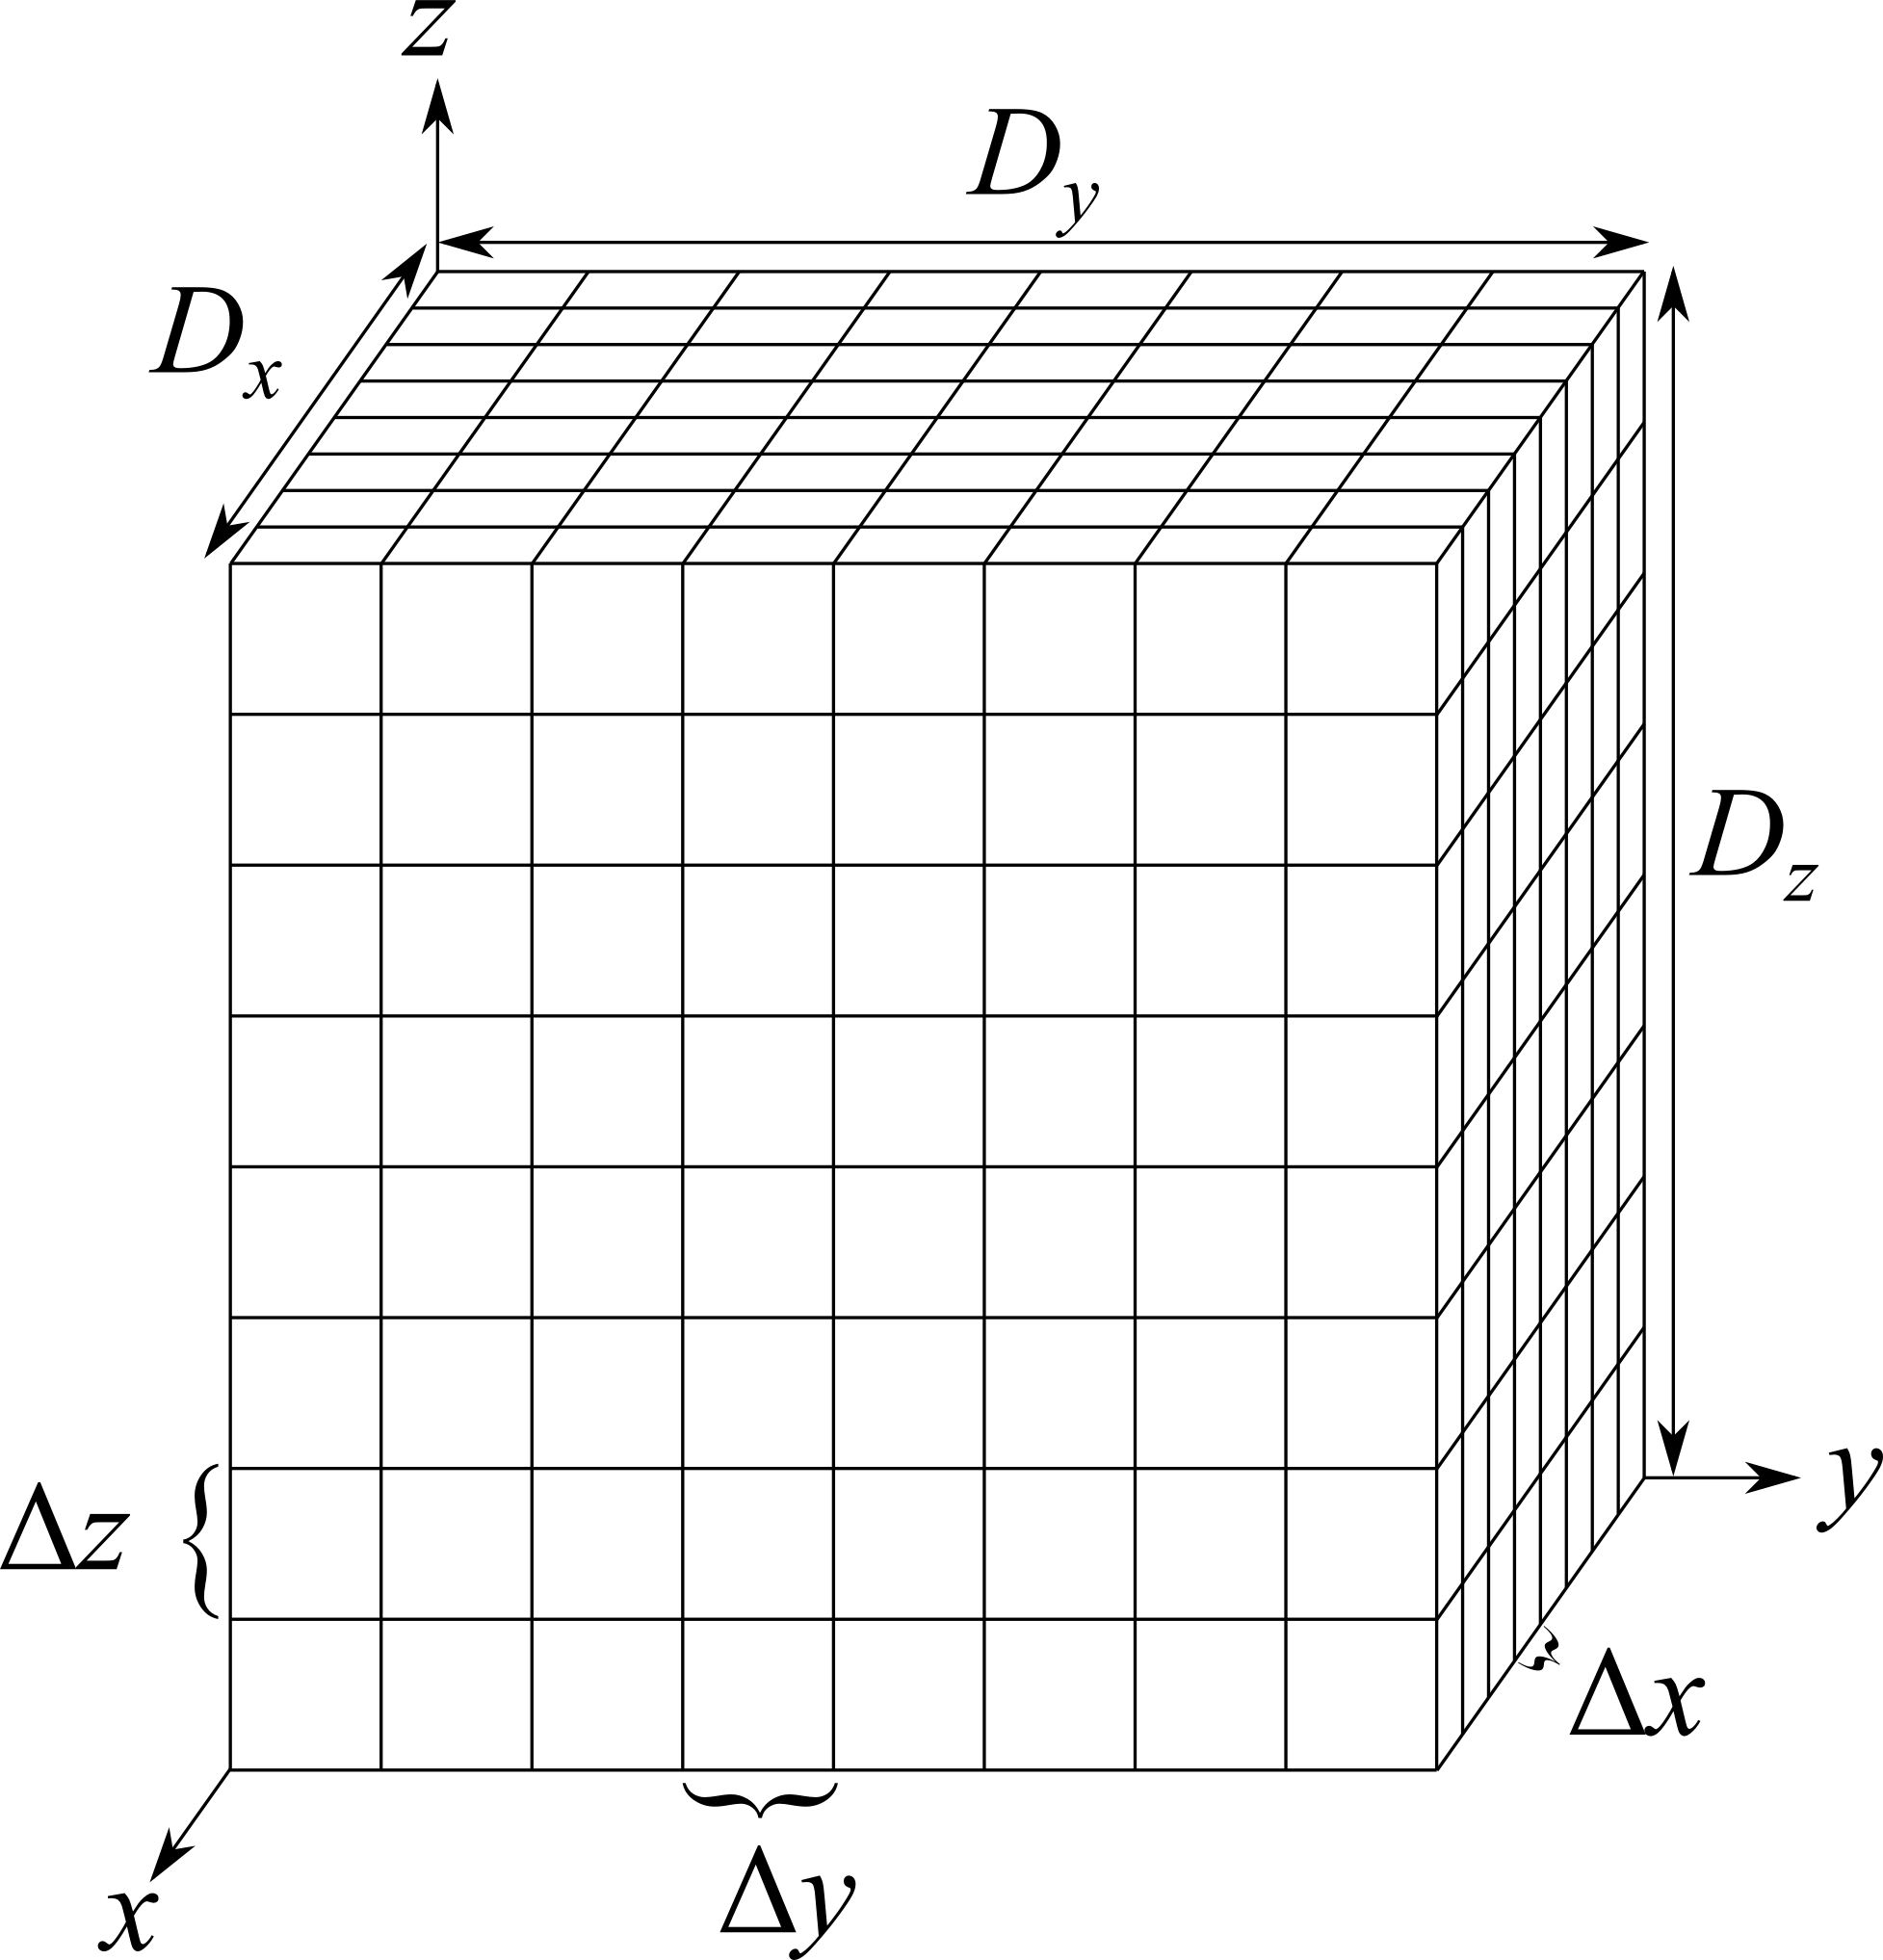
\includegraphics[width=3.75in]{figs/spatial_disc}
  \end{center}
  \caption{The spatial mesh imposed on the problem domain.}
\label{fig:spatial_disc}
\end{figure}%

The index of interest is denoted as a subscript $i$ which makes the fully discretized form of the steady state Linear Boltzmann Equation given in Eq.~\ref{eq:boltz} into the fully discretized form given in Eq.~\ref{eq:boltz_i}

\begin{equation} \label{eq:boltz_i}
\left[ \hat{\Omega}_a \cdot \nabla + \Sigma_{t,i}^g \right]
\psi_{i,a}^{g} = 
\sum_{a=0}^{N_a-1} \sum_{g'=g}^{G-1} \Sigma_{s, i, a, a'}^{g, g'} \psi_{i, a'}^{g'} \omega_a + S_{i,a}^g
\end{equation}

\subsection{Solution}

To solve the fully discretized form of the Linear Boltzmann Equation given in Eq.~\ref{eq:boltz_i}, the gradient operator must first be computed numerically. Recall that $\Omega_a$ can be written in vector notation using its cosine components as defined in Eq.~\ref{eq:omega_cos}. Also recall the definition of the gradient, given in Eq.~\ref{eq:grad}.

\begin{equation} \label{eq:grad}
\nabla f(x, y, z) = \frac{\partial f(x, y, z)}{\partial x} \hat{i} + \frac{\partial f(x, y, z)}{\partial y} \hat{j} + \frac{\partial f(x, y, z)}{\partial z} \hat{k}
\end{equation}

To the first order, a partial derivitive can be computed using Eq.~\ref{eq:deriv_1}.

\begin{equation} \label{eq:deriv_1}
\frac{\partial f(x)}{\partial x} \approx \frac{f(x) - f(x + \Delta x)}{\Delta x}
\end{equation}

Using the definition of $\Omega$ and Eq.~\ref{eq:grad} the $\hat{\Omega} \cdot \nabla \psi$ term can be rewritten using Eq.~\ref{eq:spatial_1}

\begin{equation} \label{eq:spatial_1}
\begin{split}
\Omega \cdot \nabla \psi & \approx 
\left\langle \mu, \eta, \xi \right\rangle \cdot
\left\langle \frac{\psi(x) - \psi(x + \Delta x)}{\Delta x},
\frac{\psi(y + \Delta y) - \psi(y)}{\Delta y},
\frac{\psi(z + \Delta z) - \psi(z)}{\Delta z} \right\rangle \\
& \approx 
\frac{\psi(x + \Delta x) - \psi(x)}{\Delta x} \mu + 
\frac{\psi(y + \Delta y) - \psi(y)}{\Delta y} \eta + 
\frac{\psi(z + \Delta z) - \psi(z)}{\Delta z} \xi
\end{split}
\end{equation}

Along some direction, $\Omega$, as it enters an arbitrary voxel, it must pass through either of the sides indicated in red and exit via the other as shown in Fig.~\ref{fig:gradient}. Fig.~\ref{fig:gradient} uses the $yz$ faces of the voxel for illustration. If $\eta$ is positive, $\Omega$ will enter through the $x_i$ surface and exit through the $x_{i+1}$ surface. If $\eta$ is negative, this order will be reversed. A limitation to this methodology is that $\mu$, $\eta$, and $\xi$ are assumed to be nonzero. This is ensured as long as none of the directions in the quadrature are parallel to a major axis.

\begin{figure}[tb]
  \begin{center}
   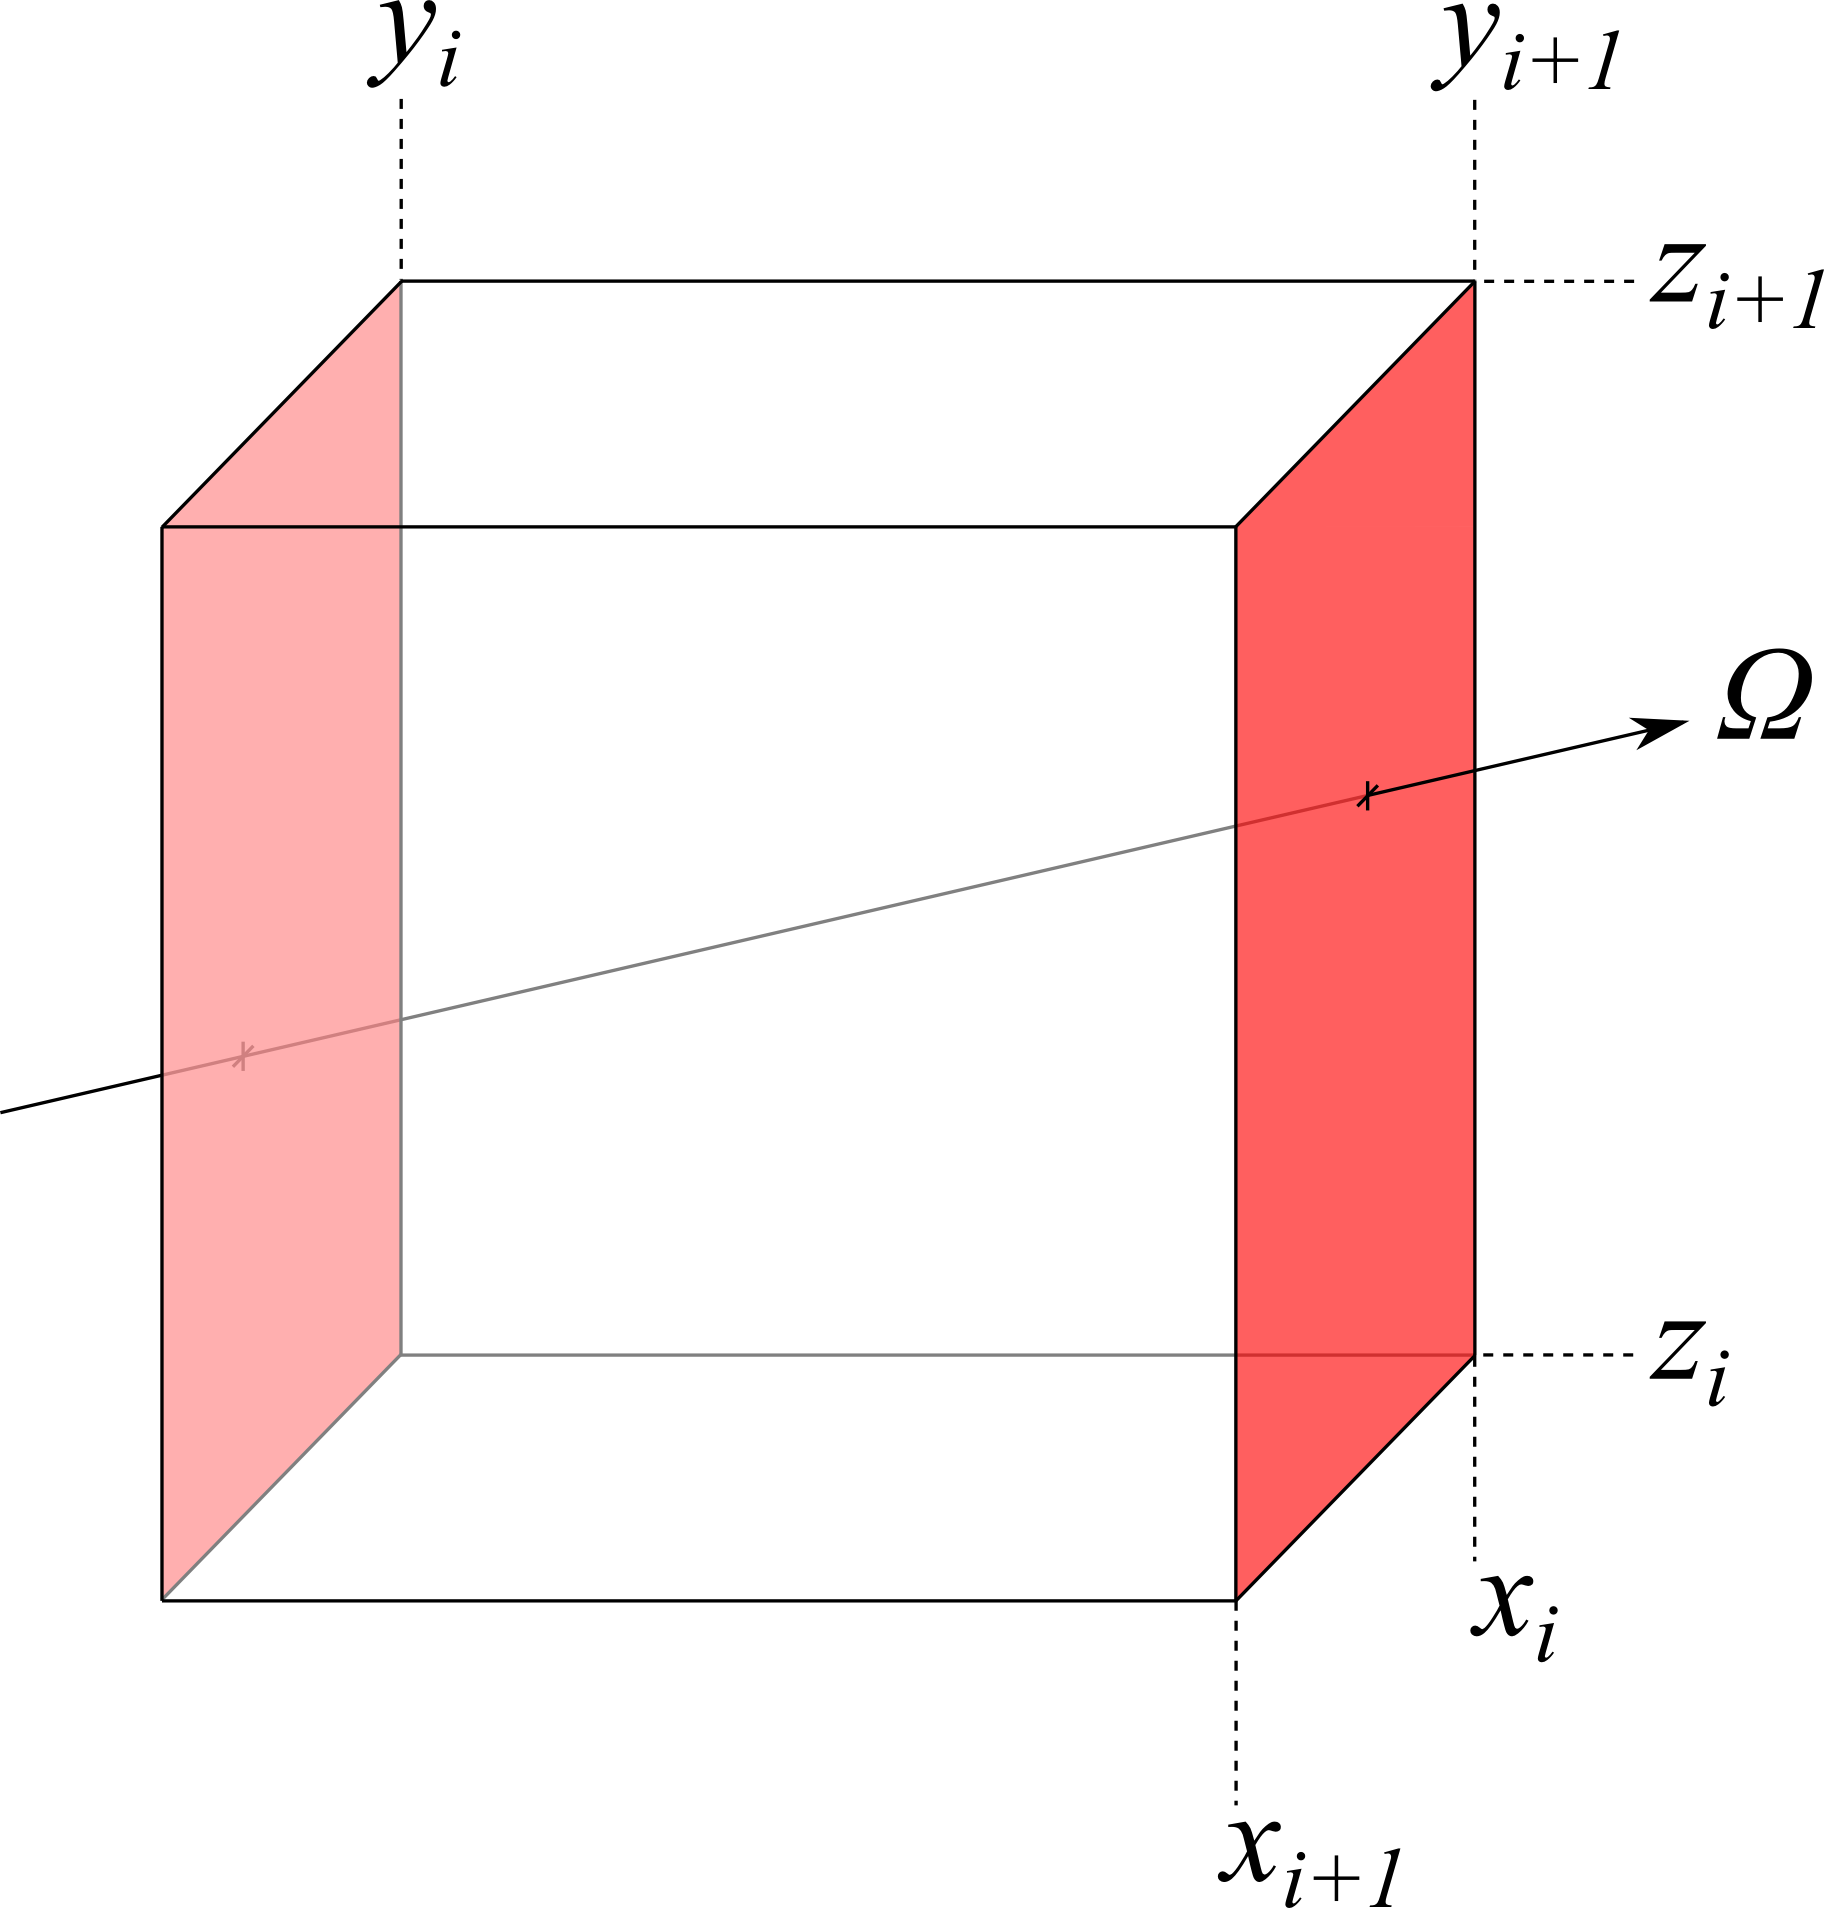
\includegraphics[width=3.75in]{figs/gradient}
  \end{center}
  \caption{The caption.}
\label{fig:gradient}
\end{figure}%

Depending on the sign of $\eta$, the first order approximation of the a derivitive along the $y$ direction is given by Eq.~\ref{eq:grad_y}.

\begin{equation} \label{eq:grad_y}
\begin{split}
\frac{\partial f}{\partial y} &= \frac{f(x_i) - f(x_{i+1})}{\Delta x}, \quad \eta>0 \\
\frac{\partial f}{\partial y} &= \frac{f(x_{i+1}) - f(x_{i})}{\Delta x}, \quad \eta <0 \\
\frac{\partial f}{\partial y} &= 0, \quad \eta=0
\end{split}
\end{equation}

Equation~\ref{eq:grad_y} can be generalized to use $f_{in}$ and $f_{out}$ instead of relying on the $x$-coordinate. This is given in Eq.~\ref{eq:grad_y2}

\begin{equation} \label{eq:grad_y2}
\begin{split}
\frac{\partial f}{\partial y} &= \frac{f_{in} - f_{out}}{\Delta x}, \quad \eta \neq 0 \\
\frac{\partial f}{\partial y} &= 0, \quad \eta=0
\end{split}
\end{equation}

The generalization of Eq.~\ref{eq:grad_y2} is applied to Eq.~\ref{eq:deriv_1} to yield Eq.~\ref{eq:deriv_2} which is generally valid for all octants.

\begin{equation} \label{eq:deriv_2}
\Omega \cdot \nabla \psi \approx 
\frac{\psi_{x,in} - \psi_{x,out}}{\Delta x} \mu + 
\frac{\psi_{y,in} - \psi_{y,out}}{\Delta y} \eta + 
\frac{\psi_{z,in} - \psi_{z,out}}{\Delta z} \xi
\end{equation}

Using the approximation given in Eq.~\ref{eq:deriv_2}, Eq.~\ref{eq:boltz_i} can be rewritten as Eq.~\ref{eq:boltz_i2}.

\begin{equation} \label{eq:boltz_i2}
\left[ 
\frac{\psi_{i,a,x,in}^g - \psi_{i,a,x,out}^g}{\Delta x} \mu + 
\frac{\psi_{i,a,y,in}^g - \psi_{i,a,y,out}^g}{\Delta y} \eta + 
\frac{\psi_{i,a,z,in}^g - \psi_{i,a,z,out}^g}{\Delta z} \xi
\right]
+ \Sigma_{t,i}^g \psi_{i,a}^{g} = 
\sum_{a=0}^{N_a-1} \sum_{g'=g}^{G-1} \Sigma_{s, i, a, a'}^{g, g'} \psi_{i, a'}^{g'} \omega_a + S_{i,a}^g
\end{equation}

It is useful to point out that each of $\psi_{i,a,x,in}^g$, $\psi_{i,a,x,out}^g$, $\psi_{i,a,y,in}^g$, $\psi_{i,a,y,out}^g$, $\psi_{i,a,z,in}^g$, and $\psi_{i,a,z,out}^g$ are \textit{surface} flux values while $\psi_{i,a}^{g}$ is a \textit{volume averaged} flux value.

In order for the discretized Linear Boltzmann Equation to be solved using Eq.~\ref{eq:boltz_i2}, the incoming flux must always be known. Either the boundary conditions or previously calculated values are used to determine each incoming flux. Therefore, in order to compute the average flux in a cell, some relationship between the average flux and the outgoing surface fluxes must be known. These values can be related by any one of many different mechanisms, the most common of which is the diamond difference approximation.

\subsection{Diamond Difference Approximation}

In the diamond difference approximation, it is assumed that the incoming and outgoing flux are both known. The average flux is assumed to be the average of the two surface fluxes. This is assumed to be the case in all three spatial dimensions. This leads to Eq.~\ref{eq:dd}.

\begin{equation} \label{eq:dd}
\begin{split}
\frac{\psi_{i,a,x,in}^g + \psi_{i,a,x,out}^g}{2} &= \psi_{i,a}^{g} \\
\frac{\psi_{i,a,y,in}^g + \psi_{i,a,y,out}^g}{2} &= \psi_{i,a}^{g} \\
\frac{\psi_{i,a,z,in}^g + \psi_{i,a,z,out}^g}{2} &= \psi_{i,a}^{g}
\end{split}
\end{equation}

Multiplying both sides of Eq.~\ref{eq:dd} and subtracting twice the outgoing surface flux from each yields Eq.~\ref{eq:dd2}.

\begin{equation} \label{eq:dd2}
\begin{split}
\psi_{i,a,x,in}^g - \psi_{i,a,x,out}^g &= 2\psi_{i,a}^{g} - \psi_{i,a,x,out}^g \\
\psi_{i,a,y,in}^g - \psi_{i,a,y,out}^g &= 2\psi_{i,a}^{g} - \psi_{i,a,y,out}^g \\
\psi_{i,a,z,in}^g - \psi_{i,a,z,out}^g &= 2\psi_{i,a}^{g} - \psi_{i,a,z,out}^g
\end{split}
\end{equation}

The form of the left hand side of Eq.~\ref{eq:dd2} is the same as in Eq.~\ref{eq:boltz_i2}. This allows Eq.~\ref{eq:dd2} to be used to make a substitution in Eq.~\ref{eq:boltz_i2} that removes the dependence on the outgoing flux from discretized equation. After the substitution, Eq.~\ref{eq:boltz_i3} will arise.

\begin{equation} \label{eq:boltz_i3}
\left[ 
\frac{2\psi_{i,a}^{g} - \psi_{i,a,x,out}^g}{\Delta x} \mu + 
\frac{2\psi_{i,a}^{g} - \psi_{i,a,y,out}^g}{\Delta y} \eta + 
\frac{2\psi_{i,a}^{g} - \psi_{i,a,z,out}^g}{\Delta z} \xi
\right]
+ \Sigma_{t,i}^g \psi_{i,a}^{g} = 
\sum_{a=0}^{N_a-1} \sum_{g'=g}^{G-1} \Sigma_{s, i, a, a'}^{g, g'} \psi_{i, a'}^{g'} \omega_a + S_{i,a}^g
\end{equation}

The diamond difference approximation defined in Eq.~\ref{eq:dd} can also be rearranged to solve for each outgoing flux once the volume averaged flux is computed. The outgoing flux is given by Eq.~\ref{eq:dd3}.

\begin{equation} \label{eq:dd3}
\begin{split}
\psi_{i,a,x,out}^g &= 2\psi_{i,a}^{g} - \psi_{i,a,x,in}^g \\
\psi_{i,a,y,out}^g &= 2\psi_{i,a}^{g} - \psi_{i,a,y,in}^g \\
\psi_{i,a,z,out}^g &= 2\psi_{i,a}^{g} - \psi_{i,a,z,in}^g
\end{split}
\end{equation}

Rearranging Eq.~\ref{eq:boltz_i3} to factor out the volume averaged flux term yields Eq.~\ref{eq:boltz_i4}.

\begin{equation} \label{eq:boltz_i4}
\left[ 
\frac{2\psi_{i,a}^{g}}{\Delta x} \mu + 
\frac{2\psi_{i,a}^{g}}{\Delta y} \eta + 
\frac{2\psi_{i,a}^{g}}{\Delta z} \xi
\right] - 
\left[ 
\frac{2\psi_{i,a,x,out}^g}{\Delta x} \mu + 
\frac{2\psi_{i,a,y,out}^g}{\Delta y} \eta + 
\frac{2\psi_{i,a,z,out}^g}{\Delta z} \xi
\right]
+ \Sigma_{t,i}^g \psi_{i,a}^{g} = 
\sum_{a=0}^{N_a-1} \sum_{g'=g}^{G-1} \Sigma_{s, i, a, a'}^{g, g'} \psi_{i, a'}^{g'} \omega_a + S_{i,a}^g
\end{equation}

Equation~\ref{eq:boltz_i4} can be directly solved for the volume averaged flux. The result is given in Eq.~\ref{eq:boltz_i5}.

\begin{equation} \label{eq:boltz_i5}
\psi_{i,a}^{g} = 
\frac{
  \sum_{a=0}^{N_a-1} \sum_{g'=g}^{G-1} \Sigma_{s, i, a, a'}^{g, g'} \psi_{i,     a'}^{g'} \omega_a + 
  \left[ 
    \frac{2\psi_{i,a,x,out}^g}{\Delta x} \mu + 
    \frac{2\psi_{i,a,y,out}^g}{\Delta y} \eta + 
    \frac{2\psi_{i,a,z,out}^g}{\Delta z} \xi
  \right] + S_{i,a}^g
}{
  \frac{2\mu}{\Delta x}  + 
  \frac{2\eta}{\Delta y} + 
  \frac{2\xi}{\Delta z} + 
  \Sigma_{t,i}^g
}
\end{equation}

\subsection{Anisotropy Treatment}

Scatter is assumed to be a function of only the scatter angle between the initial and scattered directions, $\theta_s$. Often, the cosine of the scatter angle, $\mu_s$ is used.

\begin{figure}[tb]
  \begin{center}
   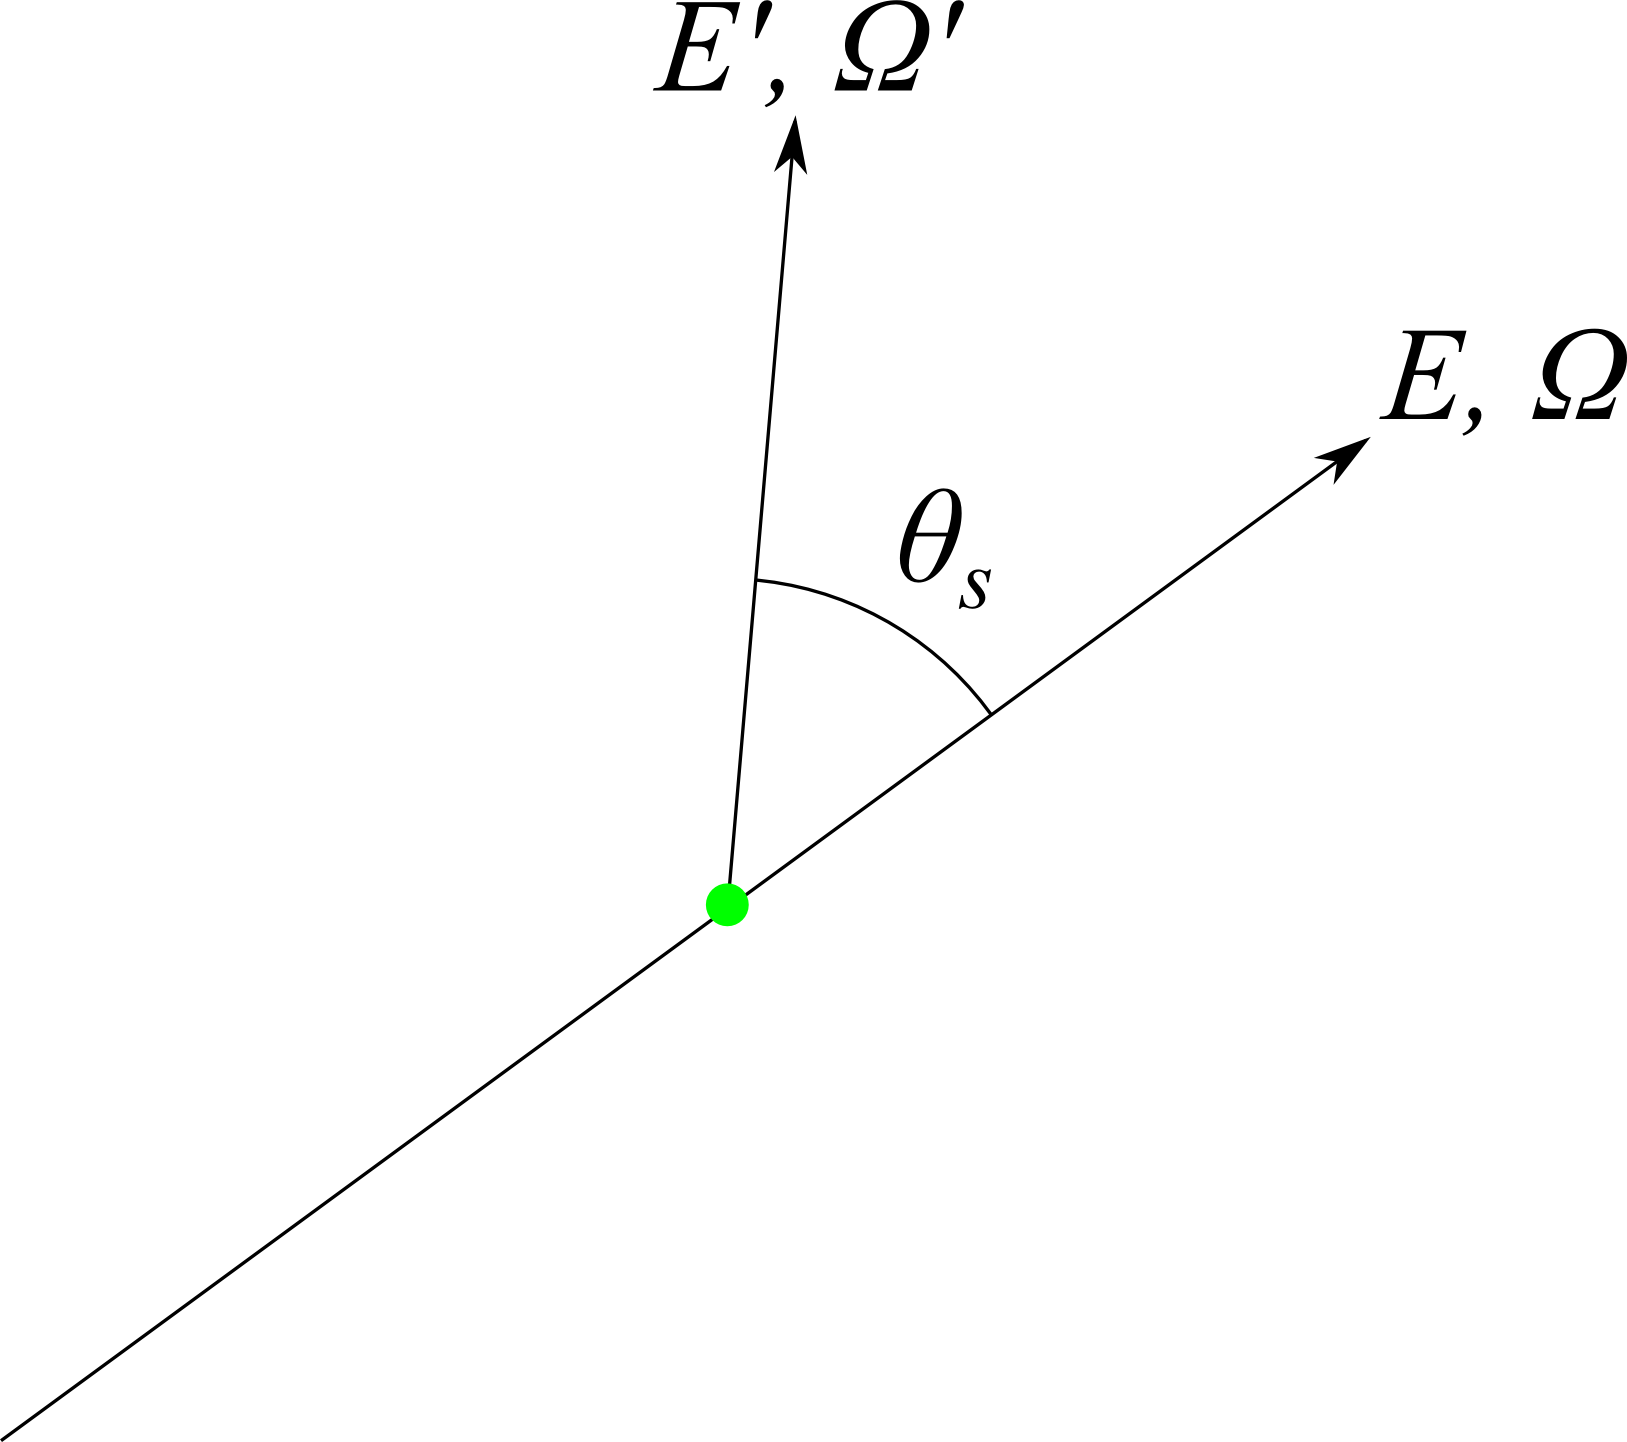
\includegraphics[width=3.75in]{figs/scat_ang}
  \end{center}
  \caption{The scatter angle. A photon at energy $E$ traveling in direction $\Omega$, hits a stationary atom, indicated by the green circle, and scatters into a new direction $\Omega'$ with a new energy $E'$.}
\label{fig:scat_ang}
\end{figure}%

The data files containing the scatter cross sections are distributed using a Legendre polynomial expansion. The use of a Legendre expansion removes the dependence on the quadrature from the data. This allows any quadrature to work with any dataset. A $l$-order Legendre polynomial is donoted by $P_l$. The anisotropic scatter cross section can then be rewritten as a Legendre expansion given in Eq.~\ref{eq:leg_1} where the scatter cosine is defined in Eq.~\ref{eq:scat_cos}

\begin{equation} \label{eq:leg_1}
\Sigma_{s, i, a, a'}^{g, g'} = \sum_{l=0}^L \frac{2l+1}{4 \pi}\Sigma_{s, i, l}^{g, g'} P_l(\mu_s)
\end{equation}

\begin{equation} \label{eq:scat_cos}
\mu_s = \Omega_a \cdot \Omega_{a'}
\end{equation}

\section{Uncollided Flux}
To avoid ray effect, the flux is split into collided and uncollided components as shown in Eq.~\ref{eq:totflux}. Equation~\ref{eq:boltz} can be rewritten as two equations solving for the uncollided flux, $\psi_u$, and collided flux, $\psi_c$ independently. Equation~\ref{eq:unc} has no scatter term since scattered particles are not considered in the uncollided flux. The source term, $S_u$, in Eq.~\ref{eq:col} is the first collision source.

\begin{equation} \label{eq:totflux}
\psi = \psi_u + \psi_c
\end{equation}

\begin{equation} \label{eq:unc}
\left[ \hat{\Omega} \cdot \nabla + \Sigma_t(\boldsymbol{r}, E) \right]
\psi_u(\boldsymbol{r}, E, \hat{\Omega}) =  S(\boldsymbol{r}, E, \hat{\Omega})
\end{equation}

\begin{equation} \label{eq:col}
\begin{split}
	&\left[ \hat{\Omega} \cdot \nabla + \Sigma_t(\boldsymbol{r}, E) \right]
	\psi_c(\boldsymbol{r}, E, \hat{\Omega}) = \\
	&\int_{4 \pi} \int_0^\infty \Sigma_s(\boldsymbol{r}, E' \rightarrow E, \hat{\Omega}' \rightarrow \hat{\Omega}) \psi_c(\boldsymbol{r}, E', \hat{\Omega}') dE' d\hat{\Omega}' + S_{u}(\boldsymbol{r}, E, \hat{\Omega})
\end{split}
\end{equation}

The uncollided flux in Eq.~\ref{eq:unc} can be analytically solved. The solution is given in Eq.~\ref{eq:uncsol} for a known isotropic point source located at position $\boldsymbol{s}$. The $\delta$ symbol in Eq.~\ref{eq:uncsol} is the Kronecker delta given by Eq.~\ref{eq:kronecker}. 

\begin{equation} \label{eq:uncsol}
\psi_u(\boldsymbol{r}, E, \hat{\Omega}) = 
S(\boldsymbol{s}, E)
\frac{e^{-\sum_i \Sigma_{t,i} x_i}}{4\pi |\boldsymbol{r}-\boldsymbol{s}|^2}
\delta\left( \hat{\Omega}, \frac{\boldsymbol{r}-\boldsymbol{s}}{|\boldsymbol{r}-\boldsymbol{s}|^2}\right)
\end{equation}

\begin{equation} \label{eq:kronecker}
\delta(\vec{A}, \vec{B}) = 
\begin{cases}
1, \quad \mathrm{if} \ \vec{A}=\vec{B} \\
0, \quad \mathrm{otherwise}
\end{cases}
\end{equation}

Equation~\ref{eq:uncsol} can be expanded to accomodate any number of spatially distributed sources of arbitrary directionality given in Eq.~\ref{eq:uncsol2} by integrating over the entire spatial domain, $V$.

\begin{equation} \label{eq:uncsol2}
\psi_u(\boldsymbol{r}, E, \hat{\Omega}) = \iiint_{V}
S(\boldsymbol{s}, E, \hat{\Omega})
\frac{e^{-\sum_i \Sigma_{t,i} x_i}}{|\boldsymbol{r}-\boldsymbol{s}|^2}
\delta\left( \hat{\Omega}, \frac{\boldsymbol{r}-\boldsymbol{s}}{|\boldsymbol{r}-\boldsymbol{s}|^2}\right)
d \boldsymbol{s}
\end{equation}

The uncollided source term, $S_u$ in Eq.~\ref{eq:col} is computed from the uncollided flux using Eq.~\ref{eq:uncsrc}.

\begin{equation} \label{eq:uncsrc}
S_u(\boldsymbol{r}, E, \hat{\Omega}) = \int_{4\pi} \int_{0}^{\infty} 
\Sigma_s(\boldsymbol{r}, E' \rightarrow E, \hat{\Omega}' \rightarrow \hat{\Omega}) \psi_u(\boldsymbol{r}, E', \hat{\Omega}') 
dE' d\hat{\Omega}'
\end{equation}

Substituting Eq.~\ref{eq:uncsrc} into $S_u$ in Eq.~\ref{eq:col} gives Eq.~\ref{eq:col2} which simplifies to Eq.~\ref{eq:col3} by using Eq.~\ref{eq:totflux} to replace the collided and uncollided components with the total angular flux.

\begin{equation} \label{eq:col2}
\begin{split}
	&\left[ \hat{\Omega} \cdot \nabla + \Sigma_t(\boldsymbol{r}, E) \right]
	\psi_c(\boldsymbol{r}, E, \hat{\Omega}) = \\
	&\int_{4 \pi} \int_0^\infty \Sigma_s(\boldsymbol{r}, E' \rightarrow E, \hat{\Omega}' \rightarrow \hat{\Omega}) \psi_c(\boldsymbol{r}, E', \hat{\Omega}') dE' d\hat{\Omega}' + \\
	&\int_{4\pi} \int_{0}^{\infty} 
\Sigma_s(\boldsymbol{r}, E' \rightarrow E, \hat{\Omega}' \rightarrow \hat{\Omega}) \psi_u(\boldsymbol{r}, E', \hat{\Omega}') 
dE' d\hat{\Omega}'
\end{split}
\end{equation}

\begin{equation} \label{eq:col3}
\begin{split}
	&\left[ \hat{\Omega} \cdot \nabla + \Sigma_t(\boldsymbol{r}, E) \right]
	\psi_c(\boldsymbol{r}, E, \hat{\Omega}) = \\
	&\int_{4 \pi} \int_0^\infty \Sigma_s(\boldsymbol{r}, E' \rightarrow E, \hat{\Omega}' \rightarrow \hat{\Omega}) \psi(\boldsymbol{r}, E', \hat{\Omega}') dE' d\hat{\Omega}'
\end{split}
\end{equation}

\section{Source Generation}
There are many kinds of external sources implemented in this work.

\subsection{Point Source}
The simplest source implemented is an isotropic point source. This source is defined only by its position and energy distribution. The center of the cell whose flux is being computed is located at position $<C_x, C_y, C_z>$ and the point source is located at position $<S_x, S_y, S_z>$.

\subsection{Fan Source}
In addition to the values defining a point source (position $\vec{S}$ and the energy distribution) a fan source is defined by two additional parameters, $\varphi$ and $\theta$ which describe the azimuthal and polar angles subtented by the fan beam respectively. Figure~\ref{fig:fanbeam} shows $\varphi$ and $\theta$ in reference to the geometry setup. The raytracing algorithm used for the fan beam is identical to the point source raytracer except for one difference: before the raytracing is done, whether the ray falls within the fan beam is determined and any ray falling outside the fan beam is not traced, its uncollided flux is immediately set to zero.

Some voxels would be partially enclosed inside the beam. A partial acceptance value is computed for these voxels and multiplied by the final result of the raytrace.

\begin{figure}[tb]
  \begin{center}
   \includegraphics[width=3.75in]{figs/fan_rejection}
  \end{center}
  \caption{The fan.}
\label{fig:fan_rejection}
\end{figure}

First, the ray direction is projected onto the $xy$ plane giving $<S_x, S_y, 0>$ and $C_x, C_y, 0$. Then the vector from the source to the geometry center and the vector from the source to the cell center are dotted to give the cosine of the angle between them as shown in Eq.~\ref{eq:phicos}. Once $\zeta$ is computed, the condition given by Eq.~\ref{eq:phicoscon} is evaluated. If the condition is met, the angle is accepted and raytraced normally, otherwise, it is rejected immediately. Figure~\ref{fig:phi}

\begin{figure}[tb]
  \begin{center}
   \includegraphics[width=3.75in]{figs/phi}
  \end{center}
  \caption{How $\varphi$ is computed.}
\label{fig:phi}
\end{figure}

\begin{equation}\label{eq:phicos}
\cos(\zeta_\varphi) = \frac{<S_x, S_y, 0>}{\sqrt{S_x^2 + S_y^2}} \cdot \frac{<C_x, C_y, 0>}{\sqrt{C_x^2 + C_y^2}} = \frac{S_x C_x + S_y C_y}{\sqrt{S_x^2 + S_y^2} \sqrt{C_x^2 + C_y^2}}
\end{equation}

\begin{equation}\label{eq:phicoscon}
|\zeta_\varphi| < \frac{\varphi}{2}
\end{equation}

Treatment for the $\theta$ variable is similar to that of $\varphi$ except the polar angle is required instead of the azimuthal angle. This is computed using Eq.~\ref{eq:thetacos} for an arbitrary vector $\vec{\xi}$. This is used to compute the polar angle for both $\vec{S}$ and $\vec{C}$. The difference between the polar angles of the two vectors is computed using Eq.~\ref{eq:thetacos2} and then the condition given in Eq.~\ref{eq:thetacoscon} is evaluated. If the condition is not met, the ray is rejected and no raytrace is performed.

\begin{equation}\label{eq:thetacos}
\cos(\theta_\xi) = \frac{\xi_z}{\sqrt{\xi_z^2 + \xi_y^2 + \xi_z^2}}
\end{equation}

\begin{equation}\label{eq:thetacos2}
\zeta_\theta = \theta_S - \theta_C
\end{equation}

\begin{equation}\label{eq:thetacoscon}
|\zeta_\theta| < \frac{\vartheta}{2}
\end{equation}


\subsection{Multi-fan Source}
A focal point is determined. The focal spot is at the center of each fan beam. The focal spot is always assumed to be at the center of the geometry and at the same $z$ elevation as the source point.

\begin{figure}
    \centering
    \begin{subfigure}[b]{0.2\textwidth}
        \includegraphics[width=\textwidth]{figs/proj6}
        \caption{$N=6$}
        \label{fig:proj6}
    \end{subfigure}
    ~ %add desired spacing between images, e. g. ~, \quad, \qquad, \hfill etc. 
      %(or a blank line to force the subfigure onto a new line)
    \begin{subfigure}[b]{0.2\textwidth}
        \includegraphics[width=\textwidth]{figs/proj12}
        \caption{$N=12$}
        \label{fig:proj12}
    \end{subfigure}
    ~ %add desired spacing between images, e. g. ~, \quad, \qquad, \hfill etc. 
    %(or a blank line to force the subfigure onto a new line)
    \begin{subfigure}[b]{0.2\textwidth}
        \includegraphics[width=\textwidth]{figs/proj16}
        \caption{$N=16$}
        \label{fig:proj16}
    \end{subfigure}
    \begin{subfigure}[b]{0.2\textwidth}
        \includegraphics[width=\textwidth]{figs/proj24}
        \caption{$N=24$}
        \label{fig:proj24}
    \end{subfigure}
    \caption{Different numbers of fan beam projections.}\label{fig:fanproj}
\end{figure}

\begin{equation}\label{eq:xp}
x' = x \cos \theta - y \sin \theta
\end{equation}

\begin{equation}\label{eq:yp}
y' = y \cos \theta + x \sin \theta
\end{equation}

To rotate a point $(x,y)$ about an arbitrary point $(x_f, y_f)$, Eq.~\ref{eq:xp2} and~\ref{eq:yp2} are used.

\begin{equation}\label{eq:xp2}
x' = (x-x_f) \cos \theta - (y-y_f) \sin \theta + x_f
\end{equation}

\begin{equation}\label{eq:yp2}
x' = (y - y_f) \cos \theta + (x - x_f) \sin \theta + y_f
\end{equation}

\subsection{Cone Source}
Pointy!

\subsection{Multi-cone Source}
All of the pointy!

\subsection{Multileaf Collimator}
How fancy.

\endinput
%%
%% End of file `chapmin.tex'.


\ThesisBodyChapter{Implementation}%%
%% Edward T. Norris
%% Discrete Ordinates Computed Tomography Organ Dose Simulator (DOCTORS)
%% 
%% === Implementation ===
%%

This chapter covers the details of the implementation of the different components of the DOCTORS code base. The code is available from a GitHub Git repository. At the time of this writing, the repository is located at \texttt{https://github.com/eNorris/thesis} and is only available subject to special request and license agreement. An executable version is available.

The code is implemented in C++ and requires a C0x11 compliant compiler. The user interface is written using the Qt5 framework. GPU computation is performed via CUDA which must be compiled seperatly by Nvidia's proprietary compiler, \texttt{nvcc}.

\section{Vector Flattening}\label{sec:flatten}

Data is stored in large, multi-dimensional arrays. For example, the CT voxel phantom can be intuitively stored as a 3D array of floating precision values which can be easily indexed. However, DOCTORS is written such that it is extensible to GPUs. GPUs are not optimized for data stored in a multi-dimensional fashion, but rather for data stored as a single 1-dimensional array. To emulate the 3-dimensional storage arrangement of the data, indexing arithmetic is used.

On the CPU, data is stored as C++ \texttt{std::vector<T>} objects where the \texttt{T} template parameter can be either \texttt{float} or \texttt{double} depending on the precision (32 bits or 64 bits respectively) needed. The storage space available to a \texttt{std::vector<T>} object is effectively unlimited, bounded only by the host CPU's physical RAM. However, other effects such as memory fragmentation can limit the practical size of a single, continuous \texttt{std::vector<T>} object significantly. To emulate indexing of a $N_x \times N_y$ matrix, a single \texttt{std::vector<T>} is created and resized to $N_x \times N_y$ elements. The global index, $i$, in the flattened array is then
\begin{equation}
i = i_x N_y + i_y.
\end{equation}
This pattern extends to multi-dimensional matrices. For example, a $N_x \times N_y$ matrix would be globally indexed as
\begin{equation}
i = i_x N_y N_z + i_y N_z + i_z.
\end{equation}

Figure~\ref{fig:indx_ex} gives an example of the spatial indexing scheme using an $8 \times 8 \times 8$ mesh. The indicated voxel has $i_x$, $i_y$, and $i_z$ indices of 1, 5, and 6 respectively. Therefore, the index value of the highlighted voxel is $1 \times 8 \times 8 + 5 \times 8 + 6$ = 110. This flattening pattern continues to higher dimensional phase space to encompas energy and direction.

\begin{figure}[tb]
  \begin{center}
   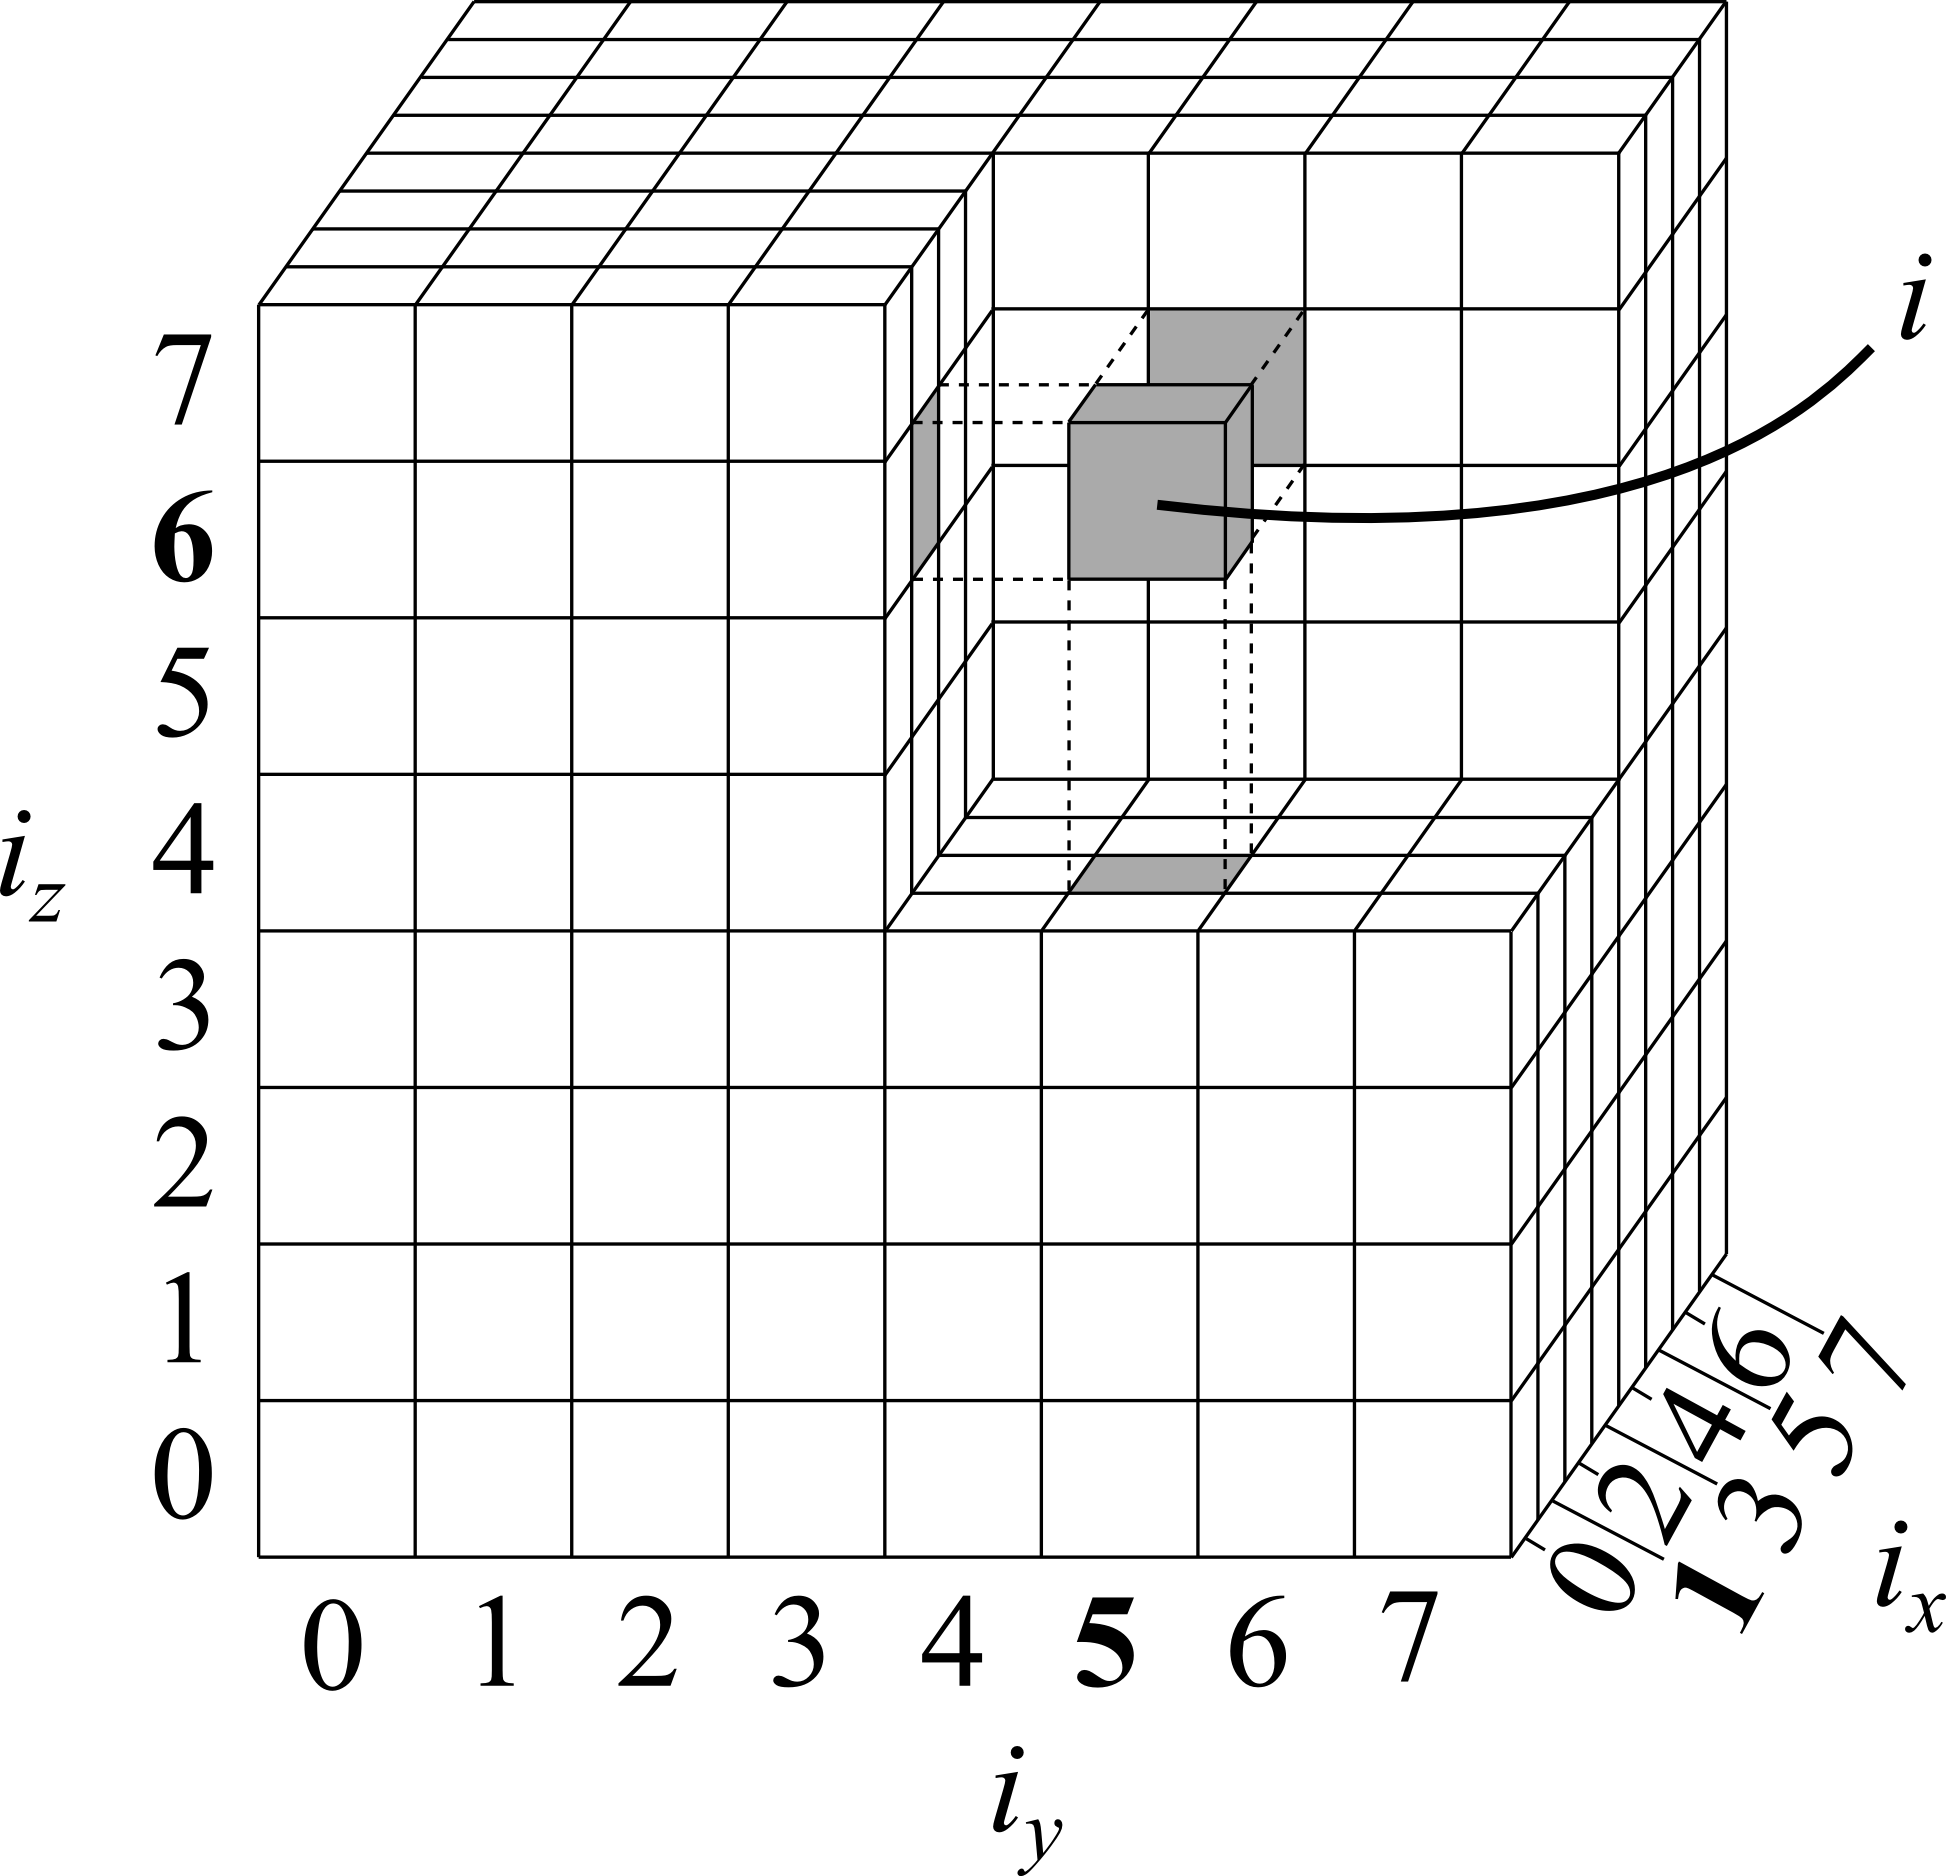
\includegraphics[width=3.75in]{figs/indx_ex}
  \end{center}
  \caption{Conversion from 3D indexing to 1D "flattened" indexing.}
\label{fig:indx_ex}
\end{figure}

A variable that is dependent on $x$, $y$, $z$, $E$, and $\Omega$ would be written as $\phi(x, y, z, E, \Omega)$ would be discretized to $\phi(i_x, i_y, i_z, G, i_a)$. Rather than storing $\phi$ as a 5-dimensional matrix, $\phi$ is stored as a 1-dimensional vector of the same number of elements.

\section{Cross Section Parsing}\label{sec:xsparse}
AMPX cross sections are stored in a binary format. Figure~\ref{fig:ampx} shows the data format of the overall file. The binary file is split into a sequence of records. The header section of the file has overall information about the file including the number of nuclides stored, their energy group structure, and a comment string describing file. Following the header section is a list of directory records. Each directory has information about a specific nuclide including the cross section reaction types available, temperatures for which the cross sections were evaluated, the number of Legendre expansion coefficients stored in the scatter matrix, and other data. Following the directories, more records follow that describe the energy structure used in the file. There is one such record for each particle type. The libraries used in the current version of DOCTORS have both neutron and photon cross section data stored.

The file header section, directories, and energy group boundaries describe the structural information necessary to read the following nuclide records. Nuclides are listed in the same order their directories are found after the header setion. Each nuclide contains numerous records.




\begin{figure}
    \centering
    \begin{subfigure}[b]{0.45\textwidth}
        \includegraphics[width=\textwidth]{figs/ampx1}
        \caption{}
        \label{fig:ampx1}
    \end{subfigure}
    ~
    \begin{subfigure}[b]{0.45\textwidth}
        \includegraphics[width=\textwidth]{figs/ampx2}
        \caption{}
        \label{fig:ampx2}
    \end{subfigure}
    \caption{The format of the AMPX file. (a) The file contains a header, a list of directory records, energy group information and a list of nuclide entries. (b) Each nuclide entry contains multiple records; the two of concern in this work are the last two containing gamma data.}\label{fig:ampx}
\end{figure}

Each record contains a string of data bytes between a four byte header and four byte footer. The header and footer are identical and, when interpreted as a signed four byte integer, give the size in bytes of the record. An example record is shown in Fig.~\ref{fig:ampxbytes1}.

The data is stored in Big Endian format which must be converted to Little Endian for most Intel and AMD processors.  The endianess rearrangement is shown in Fig.~\ref{fig:ampxbytes2}. Each record is one of 12 unique types; each type of record is formatted and interpreted differently. For example, Type 1 contains general information about the data file such as the number of nuclides, number of energy groups, and a brief description. Type 2 records contains a list of floating-point numbers representing the energy group boundaries. Figure~\ref{fig:ampxbytes1} shows a Type 1 record. In the case of the header bytes given in Fig.~\ref{fig:ampxbytes1} and~\ref{fig:ampxbytes2}, the bytes correspond to the integer 440 which is the length in bytes of the record (not including the header or footer).

Each byte of data is sequentially read, reordered, and converted to an apprpriately typed variable. Table~\ref{tab:reorder} shows the converstion for the record given in Fig.~\ref{fig:ampxbytes1}.

\begin{figure}[tb]
  \begin{center}
   \includegraphics[width=3.75in]{figs/ampxbytes1}
  \end{center}
  \caption{An example record parsed. The header and footer are identical and equal to the number of bytes in the record.}
\label{fig:ampxbytes1}
\end{figure}

\begin{figure}[tb]
  \begin{center}
   \includegraphics[width=2.75in]{figs/ampxbytes2}
  \end{center}
  \caption{The byte reordering from Big Endian to Little Endian. Individual bits within a byte are not rearranged, but the ordering of the four bytes withing a 32-bit word is reversed.}
\label{fig:ampxbytes2}
\end{figure}

\begin{table}[ht]
\caption{Byte Reordering}
\centering 
\begin{tabular}{l | c | c | c | l}
  \hline \hline   
  Word  & Big Endian & Little Endian & Interpreted & Notes\\ [0.5ex] % inserts table 
  \hline
  0   & B8 01 00 00 & 00 00 01 B8 & 440    & Header                    \\
  1   & 8B 69 00 00 & 00 00 69 8B & 27019  & ID                        \\
  2   & A4 01 00 00 & 00 00 01 A4 & 420    & Number of nuclides        \\
  ... &      ---    &      ---    &    --- & ---                       \\
  11  & 70 75 6F 43 & 43 6F 75 70 & "Coup" & First word of the title   \\
  12  & 20 64 65 6C & 6C 65 64 20 & "led " & Second word of the title  \\
  ... &     ---     &    ---      &  ---   & ---                       \\
  440 & 20 20 20 20 & 20 20 20 20 & "    " & 4 spaces ending the title \\
  441 & B8 01 00 00 & 00 00 01 B8 & 440    & Footer                    \\ 
  [1ex]      % [1ex] adds vertical space
  \hline
\end{tabular}
\label{table:reorder}
\end{table}

The header always reports the number of 8-bit bytes required to store the data. However, some data types, such as texttt{char}, are only one byte so each word represents multiple (4 in the case of \texttt{char}) distinct characters.


The first entry in each nuclide entry is the directory record. The directory contains general information regarding the nuclide and information necessary to parse the proceeding records. Following the directory, Bondarenko data, resonance parameters, neutron data, and gamma production which are not of interest in photon only problems are read.

The penultimate record contains the average cross section data. This data is averaged over all energies and directions using Eq.~\ref{eq:groupxs}. The only data used in this section in DOCTORS is the total cross section values necessary for implementing the fully discretized form of the LBE given in Eq.~\ref{eq:boltz_i}.

The 2D data is stored in a special format optimized for scatter matrix data. The format concists of a sequence of "magic numbers" interpersed within a list of data points. A magic number is a nine digit number IIIJJJKKK. The first three digits, III, are the group number of the highest energy group to scatter to the energy of interest. The next three digits, JJJ, are the group number of the lowest energy to scatter. The final three digits, KKK, are the group number of the sink energy to which particles are scattering. Given a magic number \texttt{magic}, the three values can be computed in Listing~\ref{lst:magic}. Note that the group numbers are indexed from 1 to $G$ instead of 0 to $G-1$ as required by DOCTORS. This is corrected by subtracting 1 while doing the indexing arithmetic.

\begin{listing}
\begin{minted}[frame=lines,linenos]{c++}
# Given magic
KKK = magic % 1000
JJJ = (magic % 1000000 - KKK) /1000
III = (magic - JJJ - KKK) / 1000000

src = JJJ
while src >= III
	data = READ_NEXT_BINARY_FLOAT()
	xs[(src - 1)*G + KKK - 1] = data
	src = src - 1
\end{minted}
\caption{Computation of the source and sink groups from the magic number and the subsequent data parsing.}\label{lst:magic}
\end{listing}

Figure~\ref{fig:sigmacomp} shows the microscopic cross section data pulled from the 200-neutron/47-gamma group data file currently used by DOCTORS for hydrogen and oxygen. The data is compared to reference data pulled directly from the ENDF/B-VII.1 photoatomic (MT=501) data library~\citep{ref:cullend} accessible through the Sigma database~\citep{ref:sigma}.

\begin{figure}
    \centering
    \begin{subfigure}[b]{0.45\textwidth}
        \includegraphics[width=\textwidth]{figs/sigmacomp1}
        \caption{}
        \label{fig:ampx1}
    \end{subfigure}
    ~
    \begin{subfigure}[b]{0.45\textwidth}
        \includegraphics[width=\textwidth]{figs/sigmacomp2}
        \caption{}
        \label{fig:ampx2}
    \end{subfigure}
    \caption{The microscopic cross section in bars for hydrogen and oxygen. Both subfigures show identical data, (a) shows the entire data range available in the reference data library and (b) shows only the data range applicable to DOCTORS.}\label{fig:sigmacomp}
\end{figure}

\section{Generation of Material Cross Section Data}\label{sec:xsgen}

Once the data is parsed, weighted combinations of elemental data is used to create material cross sections. Cross section data for photons always uses the naturally ocurring since photo-atomic reactions are not sensitive to the nuclear differences between isotopes. The compositions of N materials are assumed to be given as weight fractions, $w_i$ subject to
\begin{equation}
sum_{i = 1}^N w_i = 1
\end{equation}
and is converted to an atom fraction, $a_i$:
\begin{equation}
a_i = \frac{w_i}{M m_i}
\end{equation}
where
\begin{equation}
M = \sum_{i = 1}^N \frac{w_i}{m_i}
\end{equation}
and $m_i$ is the element's atomic weight.

In the solution employed by DOCTORS, only the total and scattering cross sections are required. The AMPX data files however, support arbitrary reaction types and have up to a dozen or more reactions for photo-atomic reactions alone for elemental datasets. The reaction types are identified by their MT designation. The total, inelastic, and elastic scatter cross sections are MT 501, 502, and 504 respectively. The scatter cross section used by DOCTORS is the sum of the elastic and inelastic cross sections.

The cross section of compound materials are computed as a weighted summation of their components. For example, the cross section of water for a particular reaction would be
\begin{equation}
\sigma_{H_2 O} = \frac{2 \sigma_H + \sigma_O}{3}.
\end{equation}

\begin{figure}
    \centering
    \begin{subfigure}[b]{0.45\textwidth}
        \includegraphics[width=\textwidth]{figs/airwaterxs2_19group}
        \caption{19 group data}
        \label{fig:airwaterxs2_19group}
    \end{subfigure}
    ~
    \begin{subfigure}[b]{0.45\textwidth}
        \includegraphics[width=\textwidth]{figs/airwaterxs2_47group}
        \caption{47 group data.}
        \label{fig:airwaterxs2_47group}
    \end{subfigure}
    \caption{Comparison of the group-averaged DOCTORS cross section data to continuous NIST data.}\label{fig:airwaterxs_group}
\end{figure}

\section{Qt5 Framework}\label{sec:qt}
The Qt5 framework was used for implementation of the user interface. Qt5 enables asynchronous calls through its signal/slot mechanism. Signals and slots are special functions that have additional processing performed by the meta-object-compiler (MOC). A signal can be emitted which will execute all connected slots. Signals and slots are connected manually by the user except special ones automatically generated by Qt5. 

Qt5 prvides a user interface for building user interfaces. Components such a sbuttons, drop boxes, radio buttons, etc. are made available to the user. Through extensive use of polymorphism, Qt simplifies the addition of graphical interactive elements called widgets. All widgets inherit from the base \texttt{QWidget} class which inherits from \texttt{QObject}. Any class that utilizes the signal/slot mechanism must extend the \texttt{QOjbect} class. As an example, a button can be created in the Qt5 user interface and named \texttt{button1}. This object will be accessible as \texttt{ui->button1}. When the user clicks on the button, the signal \texttt{button1.clicked()} will automatically be emitted. The user can connect this signal to any slot with an identical number arguments of the same type. The \texttt{button1.clicked()} signal can be connected to the slot \texttt{doStuff1()} but not \texttt{doStuff2(int)} since the arguments are not compatible.

Listing~\ref{lst:sync1} gives a pseudocode snippet that has a long function that will block the user interface. A corresponding dequence diagram is given in Fig.~\ref{fig:sync1}. When the user interacts with the GUI, the writer object begins executing the \texttt{doWrite()} function. Until this function completes, the UI thread will be busy an dunable to handle additionaly user interaction or updates. This results in the GUI becoming unresponsive and potentially issuing a warning to the user from the operating system.

\begin{listing}
\begin{minted}[frame=lines,linenos]{c++}
class MainWindow : public QWindow
{
	// Constructor
	MainWindow(QObject *parent);
	
	// Other parts of the class
	
public slot:
	void doSomethingLong();
}

void MainWindow::doSomethingLong()
{
	// Execute a long piece of code
}
	

MainWindow::MainWindow(QObject *parent)
{
	// Initializations
	
	// When a button named button1 which was created in the Qt5 creator interface is clicked, the clicked() signal is automatically emitted which executes the doSomethingLong() function
	MainWindow.connect(ui->button1, clicked(), this, doSomethingLong())
}
\end{minted}
\caption{A long function causes the user interface to block.}\label{lst:sync1}
\end{listing}

\begin{figure}[tb]
  \begin{center}
   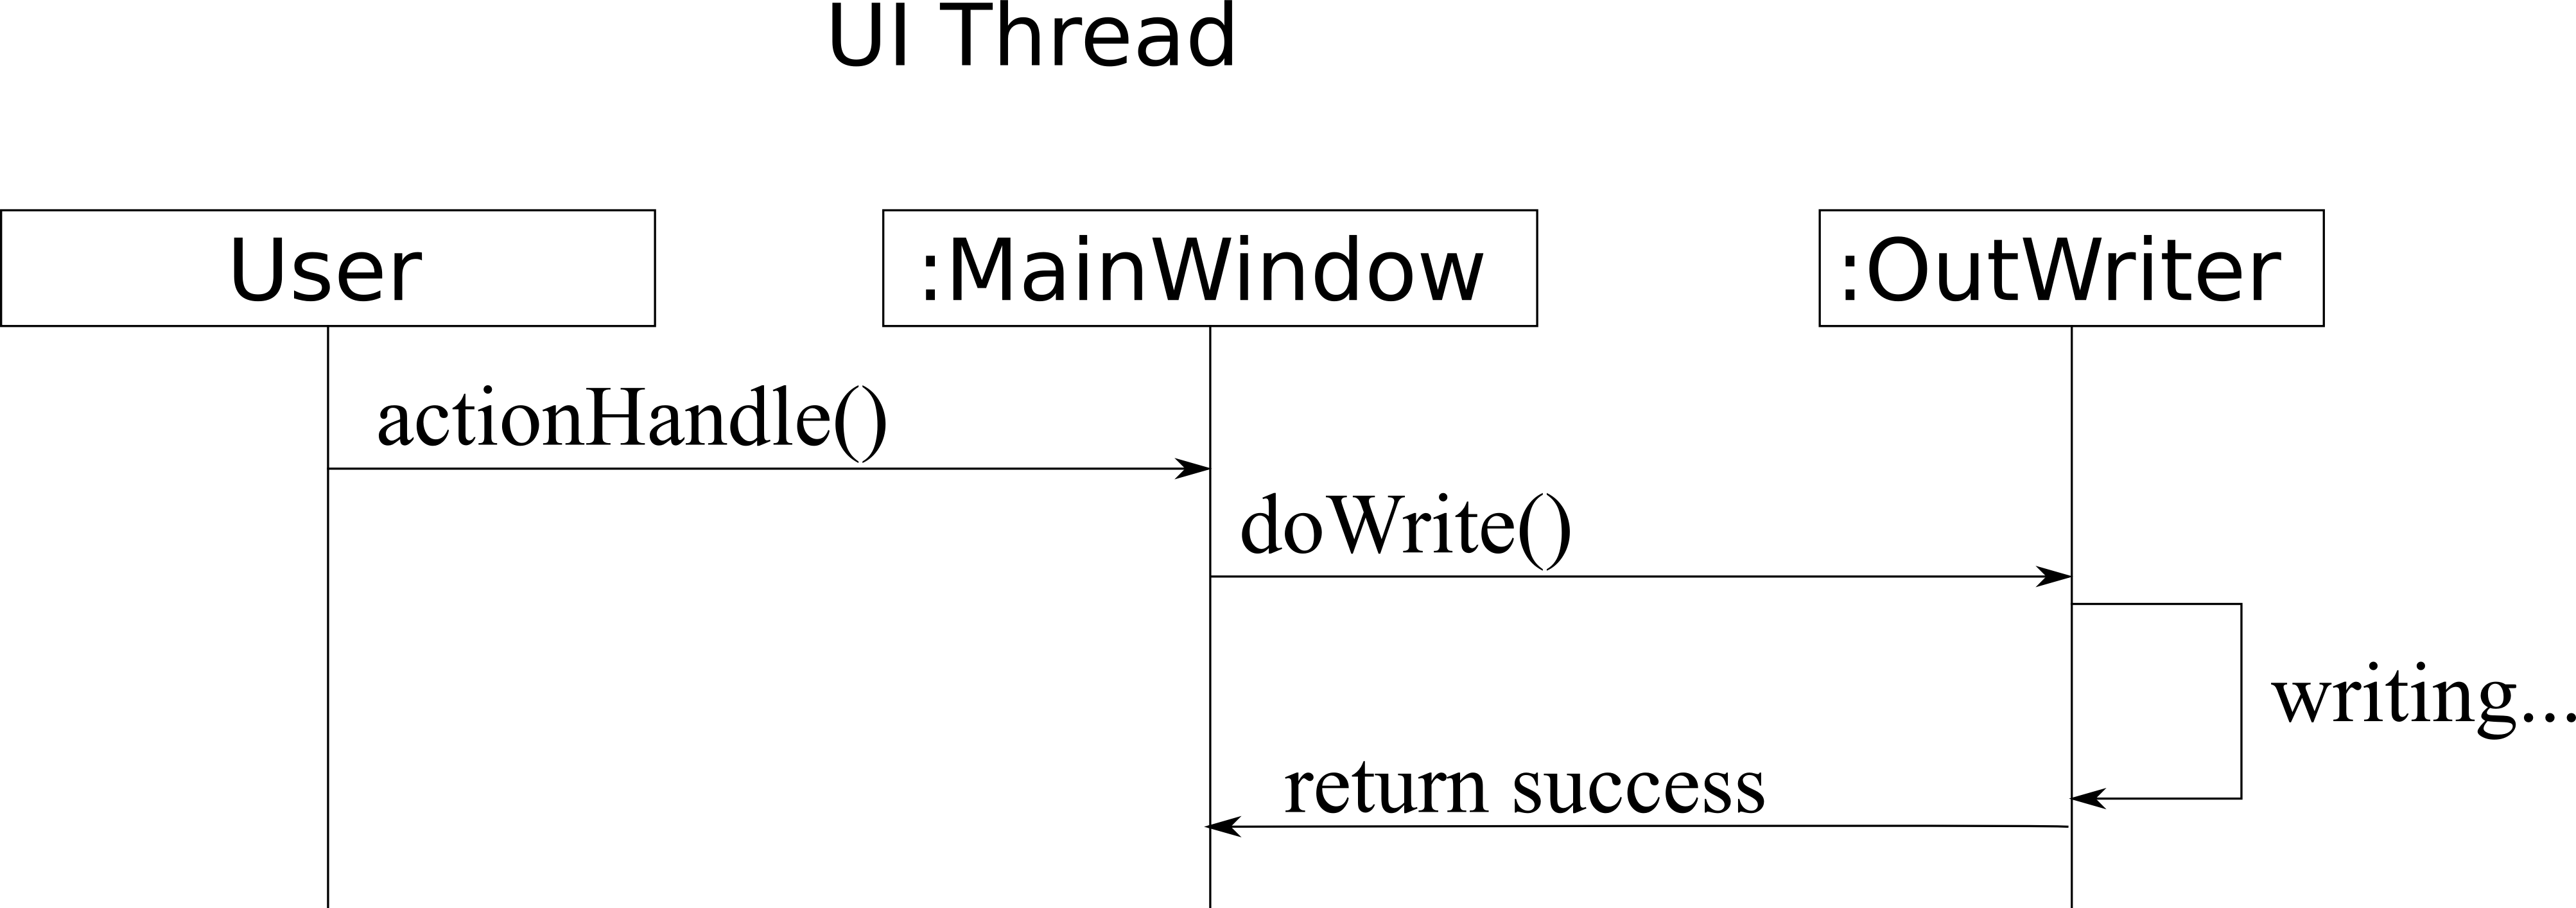
\includegraphics[width=3.75in]{figs/writer_sync}
  \end{center}
  \caption{Sequence diagram for the synchronous call.}
\label{fig:sync1}
\end{figure}%

The code in Listing~\ref{lst:sync1} is updated to use the Qt signal/slot mechanism.

\begin{listing}
\begin{minted}[frame=lines,linenos]{c++}
class MainWindow : public QWindow
{
	// Constructor
	MainWindow(QObject *parent);
	
	// Other parts of the class
	
public slot:
	void doSomethingLong();
}

void MainWindow::doSomethingLong()
{
	// Execute a long piece of code
}
	

MainWindow::MainWindow(QObject *parent)
{
	// Initializations
	
	// When a button named button1 which was created in the Qt5 creator interface is clicked, the clicked() signal is automatically emitted which executes the doSomethingLong() function
	MainWindow.connect(ui->button1, clicked(), this, doSomethingLong())
}
\end{minted}
\caption{A long function causes the user interface to block.}\label{lst:sync1}
\end{listing}

\begin{figure}[tb]
  \begin{center}
   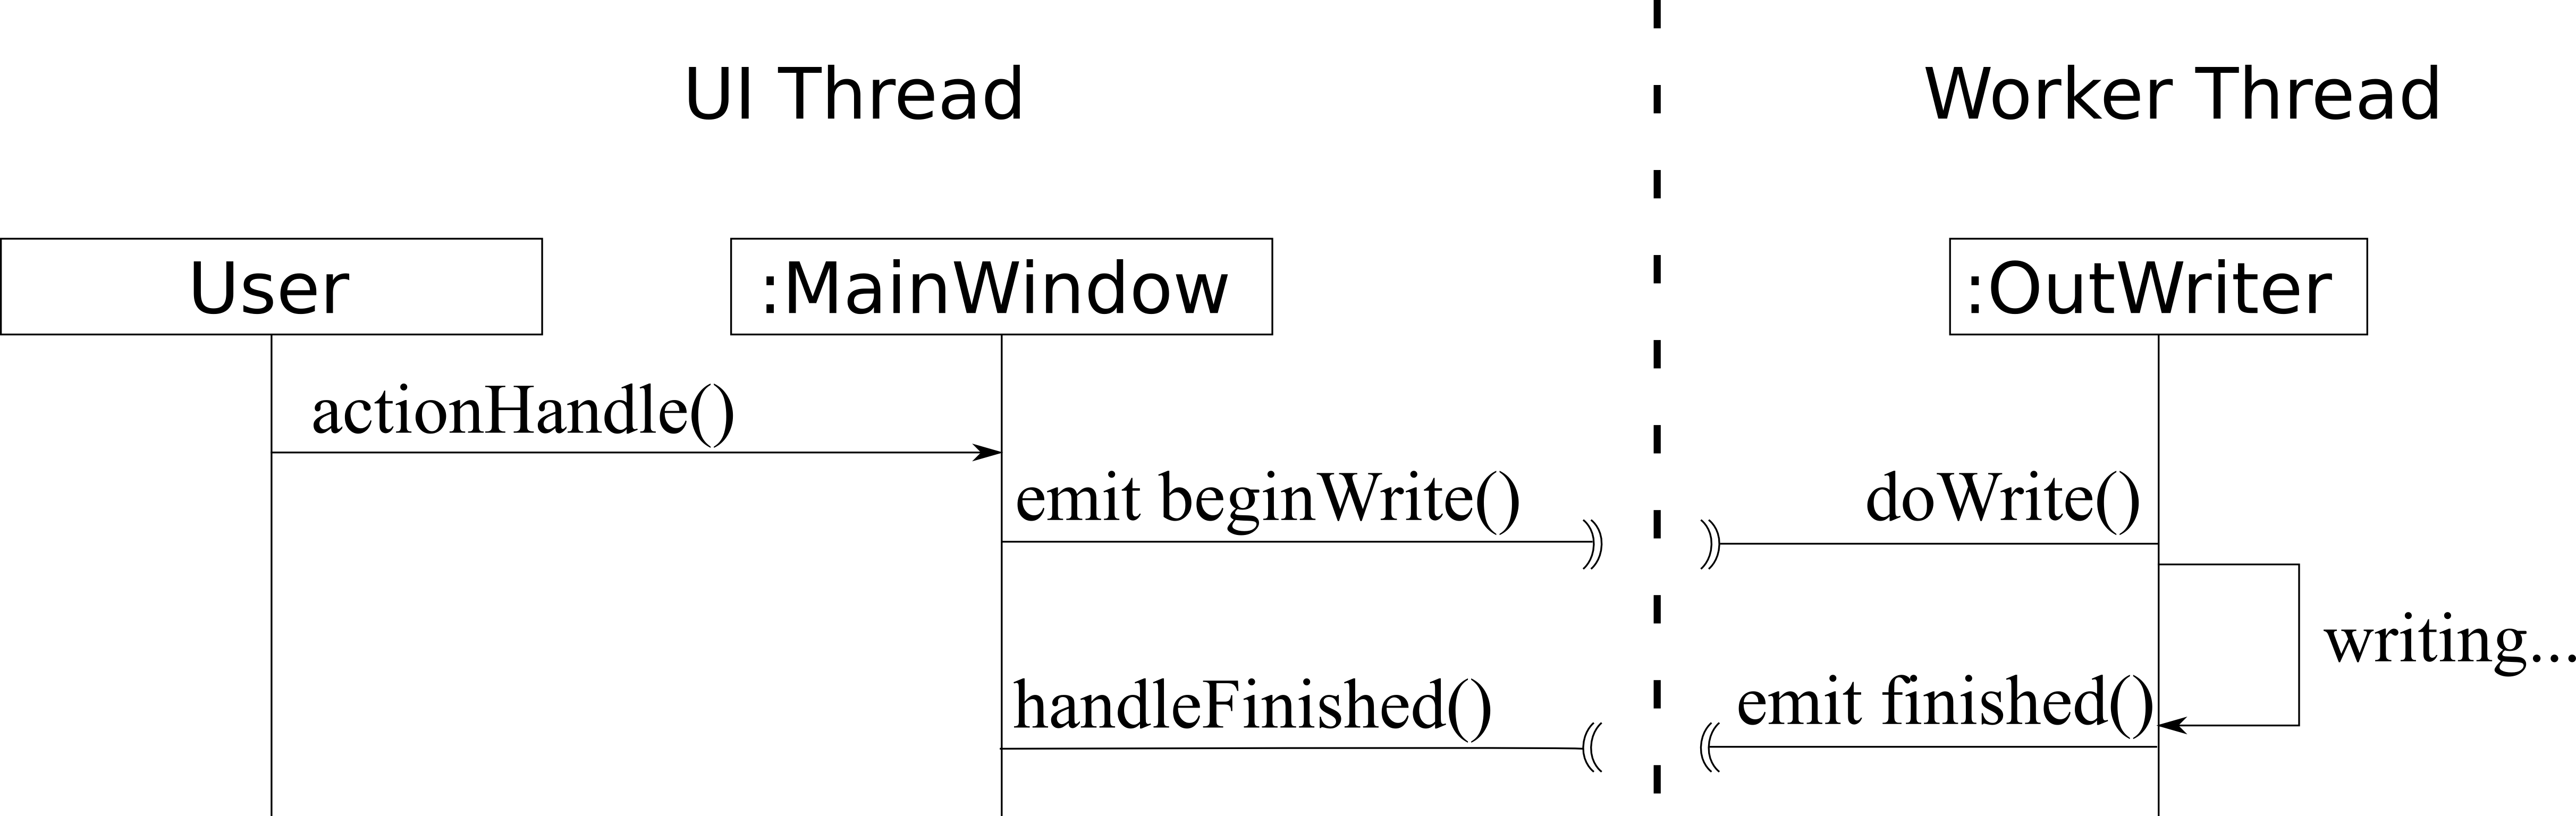
\includegraphics[width=3.75in]{figs/writer_async}
  \end{center}
  \caption{Sequence diagram for the synchronous call.}
\label{fig:async1}
\end{figure}%

\section{Graphical User Interface}\label{sec:gui}

INSERT PICTURES OF THE GUI

\section{CUDA}\label{sec:cuda}
CUDA code is compoiled with the Nvidia complier nvcc. Qt uses the gcc compiler and its MOC generator for meta code. In order to connect CUDA code to the Qt MOC, the CUDA code is compiled by nvcc to produce a .o file. Qt then compiles all other files into corresponding.o files. The linker than automactically picks up all of the .o files gneerated by nvcc. The final result is an executable that has a Qt generarted user interface that can communicat with an Nvidia graphics card through the CUDA language.

The sweep through the mesh is different.

\begin{table}[ht]
\caption{Subsweep Indices}
\centering 
\begin{tabular}{l | c | c | c | c}
  \hline \hline   
  i  & ix & iy & iz & ix+iy+iz \\ [0.5ex] % inserts table 
  \hline
  0  & 4 & 0 & 0 & 4\\
  1  & 3 & 1 & 0 & 4\\
  2  & 3 & 0 & 1 & 4\\
  3  & 2 & 2 & 0 & 4\\
  4  & 2 & 1 & 1 & 4\\
  5  & 2 & 0 & 2 & 4\\
  6  & 1 & 3 & 0 & 4\\
  7  & 1 & 2 & 1 & 4\\
  8  & 1 & 1 & 2 & 4\\
  9  & 1 & 0 & 3 & 4\\
  10 & 0 & 4 & 0 & 4\\
  11 & 0 & 3 & 1 & 4\\
  12 & 0 & 2 & 2 & 4\\
  13 & 0 & 1 & 3 & 4\\
  14 & 0 & 0 & 4 & 4\\ [1ex]      % [1ex] adds vertical space
  \hline
\end{tabular}
\label{table:subsweep}
\end{table}

We first split the sweep process into $N_L$ subsweeps. For a $N_x \times N_x \times N_x$ mesh, the subsweep process is straightforward. Some of the initial subsweeps are shown for a $8 \times 8 \times 8$ mesh in Fig.~\ref{fig:subsweep_cube}. This is valid for any direction, $\hat{\Omega}$, for which all three of its direction cosines ($\mu$, $\xi$, and $\eta$) are positive.

\begin{figure}
    \centering
    \begin{subfigure}[b]{0.45\textwidth}
        \includegraphics[width=\textwidth]{figs/subsweep_cube1}
        \caption{Subsweep 0 ($S=0$)}
        \label{fig:subsweep_cube1}
    \end{subfigure}
    ~ %add desired spacing between images, e. g. ~, \quad, \qquad, \hfill etc. 
      %(or a blank line to force the subfigure onto a new line)
    \begin{subfigure}[b]{0.45\textwidth}
        \includegraphics[width=\textwidth]{figs/subsweep_cube2}
        \caption{Subsweep 1 ($S=1$)}
        \label{fig:subsweep_cube2}
    \end{subfigure}
    ~ %add desired spacing between images, e. g. ~, \quad, \qquad, \hfill etc. 
    %(or a blank line to force the subfigure onto a new line)
    \begin{subfigure}[b]{0.45\textwidth}
        \includegraphics[width=\textwidth]{figs/subsweep_cube3}
        \caption{Subsweep 6 ($S=6$)}
        \label{fig:subsweep_cube3}
    \end{subfigure}
    \begin{subfigure}[b]{0.45\textwidth}
        \includegraphics[width=\textwidth]{figs/subsweep_cube4}
        \caption{Subsweep 6 ($S=6$) with labels}
        \label{fig:subsweep_cube4}
    \end{subfigure}
    \caption{The progression of subsweeps throughout a sweep. Each subsweep must complete before those after it. Each voxel within a subsweep can be solved in parallel with all others in its subsweep.}\label{fig:subsweep_cube}
\end{figure}

In general, blah blah.

\begin{figure}
    \centering
    \begin{subfigure}[b]{0.2\textwidth}
        \includegraphics[width=\textwidth]{figs/subsweep_general1}
        \caption{$S=0$}
        \label{fig:subsweep_general1}
    \end{subfigure}
    ~ %add desired spacing between images, e. g. ~, \quad, \qquad, \hfill etc. 
      %(or a blank line to force the subfigure onto a new line)
    \begin{subfigure}[b]{0.2\textwidth}
        \includegraphics[width=\textwidth]{figs/subsweep_general2}
        \caption{$S=1$}
        \label{fig:subsweep_general2}
    \end{subfigure}
    ~ %add desired spacing between images, e. g. ~, \quad, \qquad, \hfill etc. 
    %(or a blank line to force the subfigure onto a new line)
    \begin{subfigure}[b]{0.2\textwidth}
        \includegraphics[width=\textwidth]{figs/subsweep_general3}
        \caption{$S=2$}
        \label{fig:subsweep_general3}
    \end{subfigure}
    \begin{subfigure}[b]{0.2\textwidth}
        \includegraphics[width=\textwidth]{figs/subsweep_general4}
        \caption{$S=3$}
        \label{fig:subsweep_general4}
    \end{subfigure}
    
    \begin{subfigure}[b]{0.2\textwidth}
        \includegraphics[width=\textwidth]{figs/subsweep_general5}
        \caption{$S=4$}
        \label{fig:subsweep_general5}
    \end{subfigure}
    ~ %add desired spacing between images, e. g. ~, \quad, \qquad, \hfill etc. 
      %(or a blank line to force the subfigure onto a new line)
    \begin{subfigure}[b]{0.2\textwidth}
        \includegraphics[width=\textwidth]{figs/subsweep_general6}
        \caption{$S=5$}
        \label{fig:subsweep_general6}
    \end{subfigure}
    ~ %add desired spacing between images, e. g. ~, \quad, \qquad, \hfill etc. 
    %(or a blank line to force the subfigure onto a new line)
    \begin{subfigure}[b]{0.2\textwidth}
        \includegraphics[width=\textwidth]{figs/subsweep_general7}
        \caption{$S=6$}
        \label{fig:subsweep_general7}
    \end{subfigure}
    \begin{subfigure}[b]{0.2\textwidth}
        \includegraphics[width=\textwidth]{figs/subsweep_general8}
        \caption{$S=7$}
        \label{fig:subsweep_general8}
    \end{subfigure}
    
    \begin{subfigure}[b]{0.2\textwidth}
        \includegraphics[width=\textwidth]{figs/subsweep_general9}
        \caption{$S=8$}
        \label{fig:subsweep_general9}
    \end{subfigure}
    ~ %add desired spacing between images, e. g. ~, \quad, \qquad, \hfill etc. 
      %(or a blank line to force the subfigure onto a new line)
    \begin{subfigure}[b]{0.2\textwidth}
        \includegraphics[width=\textwidth]{figs/subsweep_general10}
        \caption{$S=9$}
        \label{fig:subsweep_general10}
    \end{subfigure}
    ~ %add desired spacing between images, e. g. ~, \quad, \qquad, \hfill etc. 
    %(or a blank line to force the subfigure onto a new line)
    \begin{subfigure}[b]{0.2\textwidth}
        \includegraphics[width=\textwidth]{figs/subsweep_general11}
        \caption{$S=10$}
        \label{fig:subsweep_general11}
    \end{subfigure}
    \begin{subfigure}[b]{0.2\textwidth}
        \includegraphics[width=\textwidth]{figs/subsweep_general12}
        \caption{$S=11$}
        \label{fig:subsweep_general12}
    \end{subfigure}
    
    \begin{subfigure}[b]{0.2\textwidth}
        \includegraphics[width=\textwidth]{figs/subsweep_general13}
        \caption{$S=12$}
        \label{fig:subsweep_general13}
    \end{subfigure}
    ~ %add desired spacing between images, e. g. ~, \quad, \qquad, \hfill etc. 
      %(or a blank line to force the subfigure onto a new line)
    \begin{subfigure}[b]{0.2\textwidth}
        \includegraphics[width=\textwidth]{figs/subsweep_general14}
        \caption{$S=13$}
        \label{fig:subsweep_general14}
    \end{subfigure}
    ~ %add desired spacing between images, e. g. ~, \quad, \qquad, \hfill etc. 
    %(or a blank line to force the subfigure onto a new line)
    \begin{subfigure}[b]{0.2\textwidth}
        \includegraphics[width=\textwidth]{figs/subsweep_general15}
        \caption{$S=14$}
        \label{fig:subsweep_general15}
    \end{subfigure}
    \caption{The generalized subsweep.}\label{fig:subsweep_general}
\end{figure}

The number of parallel tasks, $P$, that can be done on subsweep $S$ of an $N_x \times N_y \times N_z$ mesh is given by Eq.~\ref{eq:taskspersub}.

\begin{equation}\label{eq:taskspersub}
P = C_S - L_x - L_y - L_z + G_{xy} + G_{yz} + G_{xz}
\end{equation}

\begin{equation}
C_S = \frac{(S+1)(S+2)}{2}
\end{equation}

\begin{equation}
L_x = \frac{d_x(d_x+1)}{2}
\end{equation}

\begin{equation}
L_y = \frac{d_y(d_y+1)}{2}
\end{equation}

\begin{equation}
L_z = \frac{d_z(d_z+1)}{2}
\end{equation}

\begin{equation}
G_{xy} = \frac{d_{xy}(d_{xy}+1)}{2}
\end{equation}

\begin{equation}
G_{yz} = \frac{d_{yz}(d_{yz}+1)}{2}
\end{equation}

\begin{equation}
G_{xz} = \frac{d_{xz}(d_{xz}+1)}{2}
\end{equation}

\begin{equation}
d_x = \max(S+1-N_x, 0)
\end{equation}

\begin{equation}
d_y = \max(S+1-N_y, 0)
\end{equation}

\begin{equation}
d_z = \max(S+1-N_z, 0)
\end{equation}

\begin{equation}
d_{xy} = \max(S+1-N_x - Ny, 0)
\end{equation}

\begin{equation}
d_{yz} = \max(S+1-N_y - Nz, 0)
\end{equation}

\begin{equation}
d_{xz} = \max(S+1-N_x - Nz, 0)
\end{equation}

Each voxel in a subsweep can be computed in parallel. Mathematically, the $i^{th}$ subsweep from all directions can be computed in parallel. However, in practice, this results in a race condition on the GPU hardware.


DELETE BELOW HERE.

The number of elements before the 4$^{th}$ level is 1 + 2 + 3 = 6. This is simply the sum of all integers less than the level number given by Eq.~\ref{eq:levelsum}. This is conincidentally the index of the first element of that level. However, there is a special case of $N_0 = 1$.

\begin{equation} \label{eq:levelsum}
N_L = \sum_{i=1}^{L} = \frac{L(L+1)}{2}
\end{equation}

Given an index, $i$, the level to which it belongs can be computed by substituting $i$ for $N_L$ in Eq.~\ref{eq:levelsum} and solving for $L$. The index value is then floored.

\begin{equation} \label{eq:levelquadratic}
i = \frac{L(L+1)}{2} \rightarrow L^2 + L - 2i = 0
\end{equation}

\begin{equation} \label{eq:levelquadsol1}
L = \left \lfloor{\frac{-1 \pm \sqrt{1+8i}}{2}} \right \rfloor
\end{equation}

Since the index must be a positive value, the $\pm$ sign can be removed from Eq.~\ref{eq:levelquadsol1} yielding Eq.~\ref{eq:levelquadsol2}

\begin{equation} \label{eq:levelquadsol2}
L = \left \lfloor{\frac{-1 + \sqrt{1+8i}}{2}} \right \rfloor
\end{equation}

The maximum index of any level in a the $N$ subsweep is $N$. Each subsweep adds an additional level. Therefore, the ix, iy, and iz indices can be computed using Eq.~\ref{eq:levelix},~\ref{eq:leveliy}, and~\ref{eq:leveliz} respectively.

\begin{equation} \label{eq:levelix}
ix = N - N_L
\end{equation}

\begin{equation} \label{eq:leveliy}
iy = L + N_L - i
\end{equation}

\begin{equation} \label{eq:leveliz}
iz = L + i - N_L
\end{equation}

\section{MCNP Generation}\label{sec:mcnpgen}
DOCTORS has the capability to generate MCNP6 input files from the CT mesh data and source specification provided by the user.

\section{Hardware}\label{sec:hardware}
For this work, a computer with an Intel i7-5960X 8 core (16 hyperthreads) processor with a base clock speed of 3.X GHz and an Nvidia Titan Z graphics card was used. Currently, if the problem requires more memory than is available on the GPU, the problem can still be solved, but much more time will be required to to copy overhead between the CPU and GPU. If the problem requires more memory than either the GPU or CPU can provide, an error is thrown and the simulation is not run.

CUDA is Nvidia only so AMD is not considered.

\endinput
%%
%% End of file `chapall.tex'.

 % ... conclusions chapter ...

\ThesisBodyChapter{Results}%%
%% Edward T. Norris
%% Discrete Ordinates Computed Tomography Organ Dose Simulator (DOCTORS)
%% 
%% === Results ===
%%


\section{Preprocessing}
Two computational phantoms were used for verification of the DOCTORS code.

Some preprocessing was done to each phantom before it was used in DOCTORS to provide results.

The results from DOCTORS were compared to analagous results from MCNP6. The MCNP6 reference compared to is automatically generated by DOCTORS to guarantee that the geometry and source parameters are identical. This process is described in detail in Section~\ref{sec:mcnpgen}.

First subtract 1024 to account for the unsigned 16-bit int data structure.

\subsection{Artifact Removal}
At the periphery of the computational mesh, artifacts can appear as a byproduct of the reconstruction algorithm used. Figure~\ref{fig:phantomWaterUnmodified} shows the artifacts in question in a $sy$ slice at the lowest ($z = 0$) level in the phantom. Two hundred sixty one (261) artifacts were detected in the phantom. To remove these artifacts, the CT number of any voxels whose CT number was greater than or equal to 65500 was set to 0. Figure~\ref{fig:phantomWaterModified} shows the same cross sectional plot after the artifacts are removed.

The water phantom in Fig.~\ref{fig:phantomWaterModified} can be broken into four regions: the water phantom, the container, the air, and the corner artifacts. The water phantom is the centermost region of the slice

\begin{figure}[tb]
  \begin{center}
   \includegraphics[width=3.75in]{figs/phantomWaterUnmodified}
  \end{center}
  \caption{The unmodified phantom. An $xy$ slice at $z$ index = 0.}
\label{fig:phantomWaterUnmodified}
\end{figure}

\begin{figure}[tb]
  \begin{center}
   \includegraphics[width=3.75in]{figs/phantomWaterModified}
  \end{center}
  \caption{The phantom after artifacts are removed. An $xy$ slice at $z$ index = 0.}
\label{fig:phantomWaterModified}
\end{figure}



\subsection{Gantry Handling}
In some phantom models, a gantry is present. The gantry poses a challenge since it is a highly attenuating material relative to the patient which reduces the available flux.

The CT number to material conversion developed by~\cite{ref:ottossonr} which is implemented in this work does not have an equivalent for the gantry region.

\subsection{Geometry Simplification}
The original phantom data for both the water phantom and the liver phantom are $256\times256\times64$ meshes which result in 4,194,304 total voxels. Though MCNP6 is capable of running such a mesh, the overhead of loading the mesh into memory and initiating the Monte Carlo solver can take on the order of hours. Therefore, the benchmarks were run using a simplified geometry of $64\times64\times16$ which has only 65,536 voxels. The smaller files can run to completion of $10^9$ particles within two hours.

\begin{figure}[tb]
  \begin{center}
   \includegraphics[width=3.75in]{figs/waterPhantom256}
  \end{center}
  \caption{Raw CT number data for the $256 \times 256 \times 64$ water phantom.}
\label{fig:waterPhantom256}
\end{figure}

\begin{figure}[tb]
  \begin{center}
   \includegraphics[width=3.75in]{figs/waterPhantom64}
  \end{center}
  \caption{The small one}
\label{fig:waterPhantom64}
\end{figure}

\section{Cone-Beam Water Benchmark}

The first benchmark, the cone with 19 groups is given in Fig. 1. The cross section data for the water and air regions are shown in Fig.~\ref{fig:airwater19}.

The water phantom is a 35 cm diameter water cylinder that stands 12.5 inches tall. The water is encased in a 0.5 cm thick plastic container.

\begin{table}[ht]
\caption{Water Regions}
\centering 
\begin{tabular}{l c r r}
\hline \hline   
Region    & CT Range & Voxels & Fraction (\%)\\ [0.5ex] 
\hline
Water     & $0 \leq x < 67$ & 1581199 & 37.70 \\
Container & $67 \leq x < 600$ & 81502 & 1.94 \\
Air       & $600 \leq x < 1080$ & 1650372  & 39.35 \\
Artifact  & $1080 \leq x < 65535$ & 881231 & 21.01 \\  [1ex]
\hline
\end{tabular}
\label{table:nonlin}
\end{table}

Once the artifacts are removed, the histogram is plotted. Figure~\ref{fig:waterHist} shows two versions of the water histogram, \ref{fig:waterHistLin} on a linear scale and \ref{fig:waterHistLog} on a logarithmic scale.

\begin{figure}
    \centering
    \begin{subfigure}[b]{0.45\textwidth}
        \includegraphics[width=\textwidth]{figs/waterHistogramLin}
        \caption{Linear}
        \label{fig:waterHistLin}
    \end{subfigure}
    ~
    \begin{subfigure}[b]{0.45\textwidth}
        \includegraphics[width=\textwidth]{figs/waterHistogramLog}
        \caption{Logarithmic}
        \label{fig:waterHistLog}
    \end{subfigure}
    \caption{The histogram.}\label{fig:waterHist}
\end{figure}

Due to the meshing used in CT phantoms, the spatial domain of the problem is identical for both the deterministic and Monte Carlo problems. A key difference between though is the group structure used in the group-averaged deterministic cross sections. Figure~\ref{fig:airwarerxs} shows the continuous energy macroscopic cross section for both air and water versus the discretized data used by DOCTORS. Unfortunately, the datasets used in DOCTORS originate from SCALE6.2, a light water reactor analysis code. Therefore, their upper photon energy bound is 20 MeV which is far higher than necessary for diagnostic imaging. This results in the region of interesting being discretized very roughly. In the 19-group discretization, the entire diagnostic domain is covered by only three energy groups.

\begin{figure}
    \centering
    \begin{subfigure}[b]{0.45\textwidth}
        \includegraphics[width=\textwidth]{figs/airwaterxs2_19group}
        \caption{19 Groups}
        \label{fig:airwaterxs19}
    \end{subfigure}
    ~
    \begin{subfigure}[b]{0.45\textwidth}
        \includegraphics[width=\textwidth]{figs/airwaterxs2_47group}
        \caption{47 Groups}
        \label{fig:airwaterxs47}
    \end{subfigure}
    \caption{Comparison of the group cross section data used by DOCTORS to the continuous cross section data used by MCNP6. The continuous data is provided by NIST !!!CITE!!!.}\label{fig:airwaterxs}
\end{figure}


The detailed flux distribution from MCNP6 and the solver are not included here, they are provided in Appendix~\ref{sec:appc_benchmark}.

\begin{figure}
    \centering
    \begin{subfigure}[b]{0.45\textwidth}
        \includegraphics[width=\textwidth]{figs/bench_cone1_comp}
        \caption{10 - 20 MeV.}
        \label{fig:bench_cone1_comp}
    \end{subfigure}
    ~
    \begin{subfigure}[b]{0.45\textwidth}
        \includegraphics[width=\textwidth]{figs/bench_cone1_lineout}
        \caption{10 - 20 MeV lineout.}
        \label{fig:bench_cone1_lineout}
    \end{subfigure}
    
    \begin{subfigure}[b]{0.45\textwidth}
        \includegraphics[width=\textwidth]{figs/bench_cone1_comp_g17}
        \caption{100 - 200 keV.}
        \label{fig:bench_cone1_comp_g17}
    \end{subfigure}
    ~
    \begin{subfigure}[b]{0.45\textwidth}
        \includegraphics[width=\textwidth]{figs/bench_cone1_lineout_g17}
        \caption{100 - 200 keV lineout.}
        \label{fig:bench_cone1_lineout_g17}
    \end{subfigure}
    
    \begin{subfigure}[b]{0.45\textwidth}
        \includegraphics[width=\textwidth]{figs/bench_cone1_comp_g18}
        \caption{45 - 100 keV.}
        \label{fig:bench_cone1_comp_g18}
    \end{subfigure}
    ~
    \begin{subfigure}[b]{0.45\textwidth}
        \includegraphics[width=\textwidth]{figs/bench_cone1_lineout_g18}
        \caption{45 - 100 keV lineout.}
        \label{fig:bench_cone1_lineout_g18}
    \end{subfigure}
    
    \begin{subfigure}[b]{0.45\textwidth}
        \includegraphics[width=\textwidth]{figs/bench_cone1_comp_g19}
        \caption{10 - 45 keV.}
        \label{fig:bench_cone1_comp_g19}
    \end{subfigure}
    ~
    \begin{subfigure}[b]{0.45\textwidth}
        \includegraphics[width=\textwidth]{figs/bench_cone1_lineout_g19}
        \caption{10 - 45 keV lineout.}
        \label{fig:bench_cone1_lineout_g19}
    \end{subfigure}
    \caption{Comparison of the MCNP6 results and the raytracer.}\label{fig:waterHist}
\end{figure}

\begin{figure}
    \centering
    \begin{subfigure}[b]{0.45\textwidth}
        \includegraphics[width=\textwidth]{figs/bench_cone1_centerdiff}
        \caption{}
        \label{fig:bench_cone1_centerdiff}
    \end{subfigure}
    ~
    \begin{subfigure}[b]{0.45\textwidth}
        \includegraphics[width=\textwidth]{figs/bench_cone1_centerdiff2}
        \caption{}
        \label{fig:bench_cone1_centerdiff2}
    \end{subfigure}
    \caption{Comparison}\label{fig:bench_cone1_centerdifffig}
\end{figure}

\section{3 Cone-Beam Water Benchmark}

Now there are three

\section{16 Cone-Beam Water Benchmark}

And now 16.

\section{1 Cone-beam Phantom Benchmark}

It's a person!

\section{16 Cone-beam Phantom Benchmark}

It's a person!

\section{GPU Acceleration}

it's faster!


\endinput
%%
%% End of file `chapmin.tex'.
 
 
\ThesisBodyChapter{Conclusions}%%
%% This is file `chapmin.tex',
%% generated with the docstrip utility.
%%
%% The original source files were:
%%
%% ths.dtx  (with options: `chapmin')
%% 
%% IMPORTANT NOTICE:
%% 
%% For the copyright see the source file.
%% 
%% Any modified versions of this file must be renamed
%% with new filenames distinct from chapmin.tex.
%% 
%% For distribution of the original source see the terms
%% for copying and modification in the file ths.dtx.
%% 
%% This generated file may be distributed as long as the
%% original source files, as listed above, are part of the
%% same distribution. (The sources need not necessarily be
%% in the same archive or directory.)


 %% ... sample chapter ...

Conclusions.

\section{First conclusion}

I concluded many things.

\section{Future Work}

A number of simple modifications to DOCTORS could be made that would greatly increase the code's usability and robustness. One of these modifications, generation of more refined group structures, is not a change to DOCTORS \textit{per se} but rather a change in the input cross section data. The other changes are additions to DOCTORS that would add new capabilities to the software.

In addition to specific modifications, some additional, broader future goals can also be identified.

\subsection{Group Structure}

The cross section data currently used by DOCTORS are taken from SCALE6.2. While these cross sections have been found to be sufficient to produce flux distributions in medical CT imaging, a more refined group structure designed for medical applications would be worth investigation.

This work can be done using either NJOY [CITE] or the newly released AMPX [CITE] code. Either code has the capability to collapse an ENDF formatted data file into a group structure of the user's choosing in the format DOCTORS reads.



NJOY or AMPX.

\subsection{Temporal Extension}

Use 4D CT to do temporal stuff as well as spatial stuff.

\subsection{Multileaf Collimation}
Collimators!

\endinput
%%
%% End of file `chapmin.tex'.


\end{ThesisBody}
 % ... appendix - specify number of appendix chapters ...

\begin{ThesisAppendix}{two}
\ThesisAppendixChapter{Legendre Polynomials and Spherical Harmonics}%%
%% Edward T. Norris
%% Discrete Ordinates Computed Tomography Organ Dose Simulator (DOCTORS)
%% 
%% === Appendix A ===
%%

This appendix gives a brief summary of flux moments and the Legendre spherical harmonics needed to compute them.

\section{Flux Moments}\label{appdx:moments}

The flux moments are an alternate representation of the angular flux  within a system. The rationale behind usage of flux moments is that they map the discrete flux ($\psi$) from a function of angle to a function of $P_N$ expansion. This reduces the amount of memory required for computation. Storing $\psi$ directly requires storing $G \times N_V \times N_a$ values where $G$ is the number of groups, $N_V$ is the number of voxels, and $N_a$ is the number of angles. Storing the flux moments, however, requires storing only $G \times N_V \times (N^2 + 2N + 1)$ values where $N$ is the $P_N$ expansion value. For example, a problem requiring $S_6$ needs $6 \times 8 = 48$ directions, but a problem requiring $P_6$ needs 49 expansion coefficients which would seem approximately eqivalent, but typical problems require far more discrete directions than expansion coefficients. Complex problems can easily require $S_{16}$ or higher but expansions above $P_5$ are rarely encountered.

\section{Legendre Polynomials}\label{appdx:leg}

The Legendre polynomials are solutions to:
\begin{equation}
\begin{split}
P_0(\mu) &= 1 \\
P_l(\mu) &= \frac{1}{2^l l!} \frac{d^l}{d\mu^l}(\mu^2 - 1)^l \,, \quad l \in \mathbb{N}
\end{split}
\end{equation}
where $\mathbb{N}$ is the set of natural numbers (1, 2, 3...). Table~\ref{tab:legendre} gives the solution of the first few Legendre polynomials. The Legendre polynomials are orthogonal on the domain $[-1, 1]$ in that
\begin{equation}
\frac{1}{2} \int_{-1}^{1} P_l(\mu) P_{l'}(\mu) d\mu = 
\begin{cases}
\frac{1}{2l+1} \,, \quad l = l'\\
0 \,, \quad \text{otherwise}
\end{cases}
\end{equation}
holds.

\begin{table}[ht]
\caption{Legendre Polynomials}
\centering 
\begin{tabular}{c c}
\hline \hline   
$P_l$    & $P_l(\mu)$ \\ [0.5ex] 
\hline
$P_0$ & 1 \\
$P_1$ & $\mu$ \\ 
$P_2$ & $\frac{1}{2}(3\mu^2 - 1)$ \\
$P_3$ & $\frac{1}{2}(5\mu^3 - 3\mu)$ \\
$P_4$ & $\frac{1}{8}(35\mu^4 - 30x^2 + 3)$ \\
$P_5$ & $\frac{1}{8}(63\mu^5 - 70\mu^3 + 15\mu)$ \\
$P_6$ & $\frac{1}{16}(231\mu^6 - 315^4 + 105^2 - 5)$ \\
$P_7$ & $\frac{1}{16}(429\mu^7 + 693\mu^5 - 315^3 + 35^3\mu)$ \\[1ex]
\hline
\end{tabular}
\label{tab:legendre}
\end{table}

The orthogonality of the Legendre polynomials allows an infinite series to exactly represent any function on the domain $[-1, 1]$ as
\begin{equation}
f(\mu) = \sum_{l=0}^{\infty} C_l P_l(\mu)
\end{equation}
with apprpriately selected constants, $C_l$ and is used to approximate functions arbitrarily
\begin{equation}
f(\mu) \approx \sum_{l=0}^{N} C_l P_l(\mu).
\end{equation}
The Legendre polynomials are extended into the associated Legendre polynomials which have an additional orthogonality.

\section{Associated Legendre Polynomials}\label{appdx:assoc}

The associated Legendre polynomials are defined as the solution to
\begin{equation}
\begin{split}
P_l^m(\mu) &= (-1)^m (1-\mu^2)^{m/2} \frac{d^m}{d\mu^m}P_l(\mu) \\
P_l^0(\mu) &= P_l(\mu)
\end{split}
\end{equation}
and exhibit the following orthogonality on $[-1, 1]$:
\begin{equation}
\frac{1}{2} \int_{-1}^{1} P_l^m(\mu) P_{}^{}(\mu) d\mu = 
\begin{cases}
\frac{1}{2l+1} \frac{(l+m)!}{(l-m)!} \,, \quad l=l' \text{ and } m=m'\\
0\,, \quad \text{otherwise}.
\end{cases}
\end{equation}
The spherical harmonics take advantage of the double orthogonality to approximate 2D distributions.

\section{Spherical Harmonics}\label{appdx:spherical}

The spherical harmonics are defined as:
\begin{equation}
Y_{lm}(\hat{\Omega}) = \sqrt{\frac{(2l+1)(l-m)!}{(l+m)!}}P_l^m(\mu)e^{e \tau m}
\end{equation}
where $\mu$ is the cosine of the angle between $\hat{\Omega}$ and the $x$-axis and $\tau$ is the rotation about the $x$-axis with respect to the $y$-axis of $\hat{\Omega}$ projected onto the $yz$ plane which can be compuated as:
\begin{equation}
\tau = \frac{\eta}{\sqrt{\eta^2 + \xi^2}}.
\end{equation}
The spherical harmonics have the orghogonality
\begin{equation}
\int_{}^{}Y_{lm}(\hat{\Omega})Y_{l'm'}^*(\hat{\Omega}) d\hat{\Omega}= 
\begin{cases}
1 \,, \quad l = l' \text{ and } m = m' \\
0 \,, \quad \text{otherwise}
\end{cases}
\end{equation}
where $Y_{lm}^*$ is the complex conjugate of $Y_{lm}$. Using the addition theorem which states
\begin{equation}
P_l(\hat{\Omega} \cdot \hat{\Omega}') = \frac{1}{2l+1}\sum_{m=-l}^{l}Y_{lm}^*(\hat{\Omega}') Y_{lm}(\hat{\Omega})
\end{equation}
gives
\begin{equation}
P_l(\hat{\Omega} \cdot \hat{\Omega}') = P_l(\mu)P_l(\mu') + 2\sum_{m=1}^{l}\frac{(l-m)!}{(l+m)!}P_l^m(\mu) P_l^m(\mu') cos(m[\tau - \tau']).
\end{equation}

\endinput
%%
%% End of file `chapmin.tex'.


\ThesisAppendixChapter{Code Listings}%%
%% This is file `chapmin.tex',
%% generated with the docstrip utility.
%%
%% The original source files were:
%%
%% ths.dtx  (with options: `chapmin')
%% 
%% IMPORTANT NOTICE:
%% 
%% For the copyright see the source file.
%% 
%% Any modified versions of this file must be renamed
%% with new filenames distinct from chapmin.tex.
%% 
%% For distribution of the original source see the terms
%% for copying and modification in the file ths.dtx.
%% 
%% This generated file may be distributed as long as the
%% original source files, as listed above, are part of the
%% same distribution. (The sources need not necessarily be
%% in the same archive or directory.)


 %% ... sample chapter ...

The Appendix is good!

\section{Mathmatic Development}

Where does this text go?

\subsection{The Boltzmann Equation}

The time

\endinput
%%
%% End of file `chapmin.tex'.


\ThesisAppendixChapter{Benchmark Results}%%
%% This is file `chapmin.tex',
%% generated with the docstrip utility.
%%
%% The original source files were:
%%
%% ths.dtx  (with options: `chapmin')
%% 
%% IMPORTANT NOTICE:
%% 
%% For the copyright see the source file.
%% 
%% Any modified versions of this file must be renamed
%% with new filenames distinct from chapmin.tex.
%% 
%% For distribution of the original source see the terms
%% for copying and modification in the file ths.dtx.
%% 
%% This generated file may be distributed as long as the
%% original source files, as listed above, are part of the
%% same distribution. (The sources need not necessarily be
%% in the same archive or directory.)


 %% ... sample chapter ...

This appendix covers details about the benchmarks that were not included.

\section{Benchmark}\label{sec:appc_benchmark}

The cone benchmark.

\begin{figure}
    \centering
    \begin{subfigure}[b]{0.45\textwidth}
        \includegraphics[width=\textwidth]{figs/bench_cone1_mc}
        \caption{The MCNP6 flux map.}
        \label{fig:bench_cone1_mc}
    \end{subfigure}
    ~
    \begin{subfigure}[b]{0.45\textwidth}
        \includegraphics[width=\textwidth]{figs/bench_cone1_mcunc}
        \caption{The MCNP6 uncertainty.}
        \label{fig:bench_cone1_mcunc}
    \end{subfigure}
    
    \begin{subfigure}[b]{0.45\textwidth}
        \includegraphics[width=\textwidth]{figs/bench_cone1_ray}
        \caption{The raytracer solution.}
        \label{fig:bench_cone1_ray}
    \end{subfigure}
    ~
    \begin{subfigure}[b]{0.45\textwidth}
        \includegraphics[width=\textwidth]{figs/bench_cone1_diff}
        \caption{The difference.}
        \label{fig:bench_cone1_diff}
    \end{subfigure}
    \caption{Comparison of the raytracer results to MCNP6 for the 10-20 MeV energy group.}\label{fig:waterHist}
\end{figure}

\section{Next benchmark}



\endinput
%%
%% End of file `chapmin.tex'.


\end{ThesisAppendix}

 % ... references - comma separated list of bib files ...

\begin{ThesisBibliography}{BIBLIOGRAPHY}
\bibliographystyle{plainnat}
\bibliography{refs}
\end{ThesisBibliography}

 % ... vita ...

\begin{Vita}
Edward Norris graduated from Missouri University of Science and Technology in 2013 with a B.S. in both nuclear engineering and computer science, he is currently pursuing both a M.S. in computer science and a PhD in nuclear engineering. His PhD work is currently funded by a fellowship through the NRC. Edward was awarded the College of Engineering and Computing PhD Scholar award in 2017 for his academic achievements.

Previously he has participated in four summer internships at Sandia National Laboratories. While there, he served in various capacities ranging from cyber defense to radiation detection and neutron scatter simulation. He was largely involved with numerical simulations of radiation transport using Geant4 and MCNP6 as well as data collection.

Edward was also an active member of the Nuclear Science Design Team at Missouri University of Science and Technology. While on the team he solved radiation transport problems to facilitate the dosimetry of an inertial electrostatic confintement fusion device being constructed.


\end{Vita}

\end{document}

